% ============================================================================
%  PFE Report — Cloud-Native AI Operations Agent for CEM–CVM Intelligence
%  Student: Souhayl Guenichi | ESPRIT | Huawei Tunisia
%  Overleaf-ready — compile with pdflatex or lualatex
% ============================================================================
\documentclass[12pt,a4paper,oneside]{report}

% ── Encoding & Language ───────────────────────────────────────────────────────
\usepackage[utf8]{inputenc}
\usepackage[T1]{fontenc}
\usepackage[english]{babel}

% ── Page Geometry ─────────────────────────────────────────────────────────────
\usepackage[
  top=2.5cm, bottom=2.5cm, left=3cm, right=2.5cm,
  headheight=15pt
]{geometry}

% ── Fonts ─────────────────────────────────────────────────────────────────────
\usepackage{lmodern}
\usepackage{microtype}

% ── Graphics & Colors ─────────────────────────────────────────────────────────
\usepackage{graphicx}
\usepackage[dvipsnames,svgnames,x11names]{xcolor}
\usepackage{tikz}
\usetikzlibrary{
  shapes.geometric, arrows.meta, positioning, fit, calc,
  backgrounds, shadows, decorations.markings, matrix,
  patterns, chains, scopes
}
\usepackage{pgfplots}
\pgfplotsset{compat=1.18}

% ── Tables ────────────────────────────────────────────────────────────────────
\usepackage{booktabs}
\usepackage{tabularx}
\usepackage{multirow}
\usepackage{longtable}
\usepackage{array}

% ── Listings (code) ──────────────────────────────────────────────────────────
\usepackage{listings}
\lstset{
  basicstyle=\ttfamily\small,
  keywordstyle=\color{RoyalBlue}\bfseries,
  commentstyle=\color{ForestGreen}\itshape,
  stringstyle=\color{Crimson},
  backgroundcolor=\color{gray!5},
  frame=single,
  rulecolor=\color{gray!40},
  breaklines=true,
  numbers=left,
  numberstyle=\tiny\color{gray},
  tabsize=2,
  showstringspaces=false,
  captionpos=b,
}
\lstdefinelanguage{yaml}{
  keywords={true,false,null,y,n},
  sensitive=false,
  comment=[l]{\#},
  morecomment=[s]{/*}{*/},
  morestring=[b]',
  morestring=[b]",
}

% ── Math ──────────────────────────────────────────────────────────────────────
\usepackage{amsmath,amssymb}

% ── Hyperlinks & PDF metadata ────────────────────────────────────────────────
\usepackage[
  colorlinks=true,
  linkcolor=RoyalBlue,
  citecolor=ForestGreen,
  urlcolor=Crimson,
  bookmarks=true,
  pdfauthor={Souhayl Guenichi},
  pdftitle={Cloud-Native AI Operations Agent for CEM-CVM Intelligence},
]{hyperref}
\usepackage{bookmark}

% ── Bibliography ──────────────────────────────────────────────────────────────
\usepackage[numbers,sort&compress]{natbib}

% ── Headers & Footers ────────────────────────────────────────────────────────
\usepackage{fancyhdr}
\pagestyle{fancy}
\fancyhf{}
\fancyhead[L]{\nouppercase{\leftmark}}
\fancyhead[R]{\thepage}
\renewcommand{\headrulewidth}{0.4pt}

% ── Captions ──────────────────────────────────────────────────────────────────
\usepackage[font=small,labelfont=bf]{caption}
\usepackage{subcaption}

% ── Misc ──────────────────────────────────────────────────────────────────────
\usepackage{enumitem}
\usepackage{float}
\usepackage{pdfpages}
\usepackage{appendix}

% ── Custom Colors (Huawei palette) ───────────────────────────────────────────
\definecolor{huaweired}{HTML}{CF0A2C}
\definecolor{huaweidark}{HTML}{1A1A2E}
\definecolor{ossblue}{HTML}{2E86AB}
\definecolor{bssgreen}{HTML}{2ECC71}
\definecolor{aiviolet}{HTML}{8E44AD}
\definecolor{cvmorange}{HTML}{E67E22}
\definecolor{cemteal}{HTML}{1ABC9C}
\definecolor{datalake}{HTML}{3498DB}
\definecolor{darkbg}{HTML}{2C3E50}
\definecolor{lightgray}{HTML}{ECF0F1}

% ── TikZ Styles (reusable across all diagrams) ───────────────────────────────
\tikzset{
  % Service / component boxes
  service/.style={
    rectangle, rounded corners=4pt, minimum width=3.2cm, minimum height=1.2cm,
    draw=#1!70!black, fill=#1!15, text=black, font=\small\bfseries,
    drop shadow={shadow xshift=1pt, shadow yshift=-1pt, opacity=0.15},
    align=center, line width=0.8pt,
  },
  service/.default={ossblue},
  % Data stores
  datastore/.style={
    cylinder, shape border rotate=90, aspect=0.25,
    minimum width=2.2cm, minimum height=1.4cm,
    draw=#1!70!black, fill=#1!12, text=black, font=\small\bfseries,
    align=center, line width=0.8pt,
  },
  datastore/.default={datalake},
  % External systems
  external/.style={
    rectangle, rounded corners=2pt, minimum width=2.8cm, minimum height=1cm,
    draw=gray!60, fill=gray!8, text=black, font=\small,
    dashed, align=center, line width=0.7pt,
  },
  % Arrows
  myarrow/.style={-{Stealth[length=6pt]}, line width=0.9pt, #1},
  myarrow/.default={darkbg},
  biarrow/.style={{Stealth[length=5pt]}-{Stealth[length=5pt]}, line width=0.8pt, #1},
  biarrow/.default={darkbg},
  % Labels on arrows
  arrlabel/.style={font=\scriptsize, fill=white, inner sep=1.5pt, text=darkbg},
  % Layer boxes
  layerbox/.style={
    rectangle, rounded corners=6pt, draw=#1!50, fill=#1!5,
    inner sep=10pt, line width=1pt,
  },
  layerbox/.default={ossblue},
  % Title labels
  layertitle/.style={font=\small\bfseries\sffamily, text=#1!70!black},
  layertitle/.default={ossblue},
}

% ── Document ──────────────────────────────────────────────────────────────────
\begin{document}

% ══════════════════════════════════════════════════════════════════════════════
%  FRONT MATTER
% ══════════════════════════════════════════════════════════════════════════════

% ============================================================================
%  Chapter 0 --- Front Matter (Title Page, Dedications, Abstract)
% ============================================================================

% ── Title Page ────────────────────────────────────────────────────────────────
\begin{titlepage}
\begin{center}

\vspace*{0.5cm}

% --- University & Company logos (replace with actual files) ---
% \includegraphics[height=2cm]{images/esprit-logo.png}
% \hfill
% \includegraphics[height=2cm]{images/huawei-logo.png}

{\large\textsc{ESPRIT --- École Supérieure Privée d'Ingénierie et de Technologies}}\\[4pt]
{\small Department of Computer Science and Telecommunications}

\vspace{1.5cm}

\rule{\linewidth}{0.8pt}\\[0.6cm]
{\LARGE\bfseries Cloud-Native AI Operations Agent\\[6pt]
for CEM--CVM Intelligence}\\[0.3cm]
{\large\itshape Bridging Customer Experience Management and Customer Value Management\\
with Agentic AI on Huawei Cloud Stack}\\[0.4cm]
\rule{\linewidth}{0.8pt}

\vspace{1.5cm}

{\large\textbf{End-of-Studies Project (PFE)}\\[4pt]
Submitted in partial fulfilment of the requirements for the\\
\textbf{Engineering Degree in Computer Science / Telecommunications}}

\vspace{1.5cm}

\begin{tabular}{rl}
\textbf{Student:}     & Souhayl Guenichi \\[4pt]
\textbf{Host Company:}& Huawei Tunisia --- Cloud IT / Sales-Solution \\[4pt]
\textbf{Supervisor:}  & \textit{[Supervisor Name]} \\[4pt]
\textbf{Academic Year:}& 2025 -- 2026 \\
\end{tabular}

\vfill

{\small March 2026}

\end{center}
\end{titlepage}

% ── Dedication (optional) ────────────────────────────────────────────────────
\chapter*{Dedication}
\addcontentsline{toc}{chapter}{Dedication}
\vspace*{2cm}
\begin{center}
\textit{To my family, for their unconditional support throughout this journey.}
\end{center}
\newpage

% ── Acknowledgments ──────────────────────────────────────────────────────────
\chapter*{Acknowledgments}
\addcontentsline{toc}{chapter}{Acknowledgments}

I would like to express my sincere gratitude to:

\begin{itemize}[leftmargin=1.5cm]
  \item My supervisor at Huawei Tunisia, for his guidance on the industrial positioning of this project within the CEM--CVM--ADN ecosystem and for facilitating access to real operator data.
  \item The Huawei Cloud IT / Sales-Solution team in Tunisia, for providing the technical context of SmartCare, Customer Value Management, and the Autonomous Driving Network paradigm.
  \item Tunisie Telecom, for granting access to anonymised production OSS/BSS data that enabled real-world model training and validation.
  \item My academic supervisor at ESPRIT, for the methodological guidance and critical review throughout this project.
  \item The jury members, for the time dedicated to evaluating this work.
\end{itemize}
\newpage

% ── Abstract (English) ───────────────────────────────────────────────────────
\chapter*{Abstract}
\addcontentsline{toc}{chapter}{Abstract}

Modern telecommunications operators generate vast volumes of network performance data (OSS) and business metrics (BSS) across heterogeneous systems. However, the correlation between network degradations and their business impact---customer churn, revenue loss, SLA breaches---remains a manual, fragmented process. Huawei's Customer Experience Management platform (SmartCare) produces rich experience indicators, yet the intelligence layer that translates these signals into actionable business decisions for Customer Value Management (CVM) systems is largely absent or siloed.

This project designs and implements a \textbf{cloud-native AI Operations Agent} that fills this gap. Positioned as the intelligence bridge between CEM (SmartCare) and CVM, the platform ingests real OSS and BSS data from Tunisie Telecom, organises it through a three-layer data lake (Raw $\to$ Processed $\to$ Curated), and applies machine learning models---\texttt{GradientBoostingRegressor} for SLA risk prediction and \texttt{IsolationForest} for network and revenue anomaly detection---to produce actionable insights. An OSS--BSS correlation engine quantifies the statistical relationship between network degradation and revenue impact using Pearson and Spearman coefficients.

The entire platform is containerised with Docker Compose (five microservices: API Gateway, Pipeline Worker, AI Service, PostgreSQL, MinIO) and architecturally mapped to Huawei Cloud Stack (HCS): OBS for object storage, RDS for the relational layer, and ECS/CCE for compute. The system is framed within Huawei's \textbf{Autonomous Driving Network (ADN)} paradigm, demonstrating how an AI agent can autonomously monitor, correlate, and act upon telecom operational and business signals.

Trained on real anonymised data from a live Tunisian operator, the models deliver credible precision, recall, and F1 scores validated against known network events. The project constitutes an industrial-grade reference implementation of O+B (OSS+BSS) convergence at PFE scale.

\vspace{0.5cm}
\noindent\textbf{Keywords:} AI Operations, CEM, CVM, SmartCare, Anomaly Detection, SLA Risk Prediction, OSS--BSS Convergence, Cloud-Native, Docker, Huawei Cloud Stack, Autonomous Driving Network, Tunisie Telecom, Machine Learning, Data Lake.

\newpage

% ── Résumé (French) ──────────────────────────────────────────────────────────
\chapter*{Résumé}
\addcontentsline{toc}{chapter}{Résumé}

Les opérateurs de télécommunications modernes génèrent d'importants volumes de données de performance réseau (OSS) et de métriques métier (BSS) à travers des systèmes hétérogènes. La corrélation entre les dégradations réseau et leur impact métier --- attrition client, perte de revenus, violations de SLA --- reste un processus fragmenté et manuel. La plateforme CEM (Customer Experience Management) de Huawei, SmartCare, produit de riches indicateurs d'expérience, mais la couche d'intelligence qui traduit ces signaux en décisions actionnables pour les systèmes CVM (Customer Value Management) est en grande partie absente.

Ce projet conçoit et implémente un \textbf{Agent AI d'Opérations cloud-natif} qui comble ce vide. Positionné comme le pont d'intelligence entre CEM (SmartCare) et CVM, la plateforme ingère des données OSS et BSS réelles de Tunisie Telecom, les organise via un lac de données à trois couches (Brut $\to$ Traité $\to$ Consolidé), et applique des modèles de machine learning --- \texttt{GradientBoostingRegressor} pour la prédiction du risque SLA et \texttt{IsolationForest} pour la détection d'anomalies réseau et de revenus --- afin de produire des insights actionnables. Un moteur de corrélation OSS--BSS quantifie la relation statistique entre la dégradation réseau et l'impact sur les revenus à l'aide des coefficients de Pearson et Spearman.

L'ensemble de la plateforme est conteneurisée avec Docker Compose (cinq microservices) et architecturalement projetée sur Huawei Cloud Stack (HCS). Le système s'inscrit dans le paradigme du \textbf{Réseau Autonome (ADN)} de Huawei, démontrant comment un agent IA peut surveiller, corréler et agir de manière autonome sur les signaux opérationnels et métier des télécommunications.

\vspace{0.5cm}
\noindent\textbf{Mots-clés :} Agent IA, CEM, CVM, SmartCare, Détection d'anomalies, Prédiction de risque SLA, Convergence OSS--BSS, Cloud-Natif, Docker, Huawei Cloud Stack, Réseau Autonome, Tunisie Telecom, Apprentissage Automatique, Lac de données.

\newpage

% ── Glossary / Acronyms ─────────────────────────────────────────────────────
\chapter*{List of Acronyms}
\addcontentsline{toc}{chapter}{List of Acronyms}

\begin{longtable}{@{}ll@{}}
\toprule
\textbf{Acronym} & \textbf{Definition} \\
\midrule
\endhead
ADN   & Autonomous Driving Network \\
API   & Application Programming Interface \\
APPU  & Average Purchase Per User \\
ARPU  & Average Revenue Per User \\
BSS   & Business Support System \\
CCE   & Cloud Container Engine (Huawei) \\
CEI   & Customer Experience Index \\
CEM   & Customer Experience Management \\
CVM   & Customer Value Management \\
DOU   & Data of Use (monthly data consumption) \\
EAP   & Experience Analytics Platform \\
ECS   & Elastic Cloud Server (Huawei) \\
FTTx  & Fibre to the x (generic fibre access) \\
GBR   & Gradient Boosting Regressor \\
HCS   & Huawei Cloud Stack \\
IF    & Isolation Forest \\
IoT   & Internet of Things \\
KPI   & Key Performance Indicator \\
KQI   & Key Quality Indicator \\
NMS   & Network Management System \\
NOM   & Network Operations Management \\
O+B   & OSS + BSS (convergence) \\
OBS   & Object Storage Service (Huawei) \\
OSS   & Operations Support System \\
RAN   & Radio Access Network \\
RDS   & Relational Database Service (Huawei) \\
REST  & Representational State Transfer \\
RSRP  & Reference Signal Received Power \\
SLA   & Service Level Agreement \\
TT    & Tunisie Telecom \\
VAS   & Value Added Services \\
VPC   & Virtual Private Cloud \\
\bottomrule
\end{longtable}

\newpage


\tableofcontents
\listoffigures
\listoftables

% ══════════════════════════════════════════════════════════════════════════════
%  MAIN CHAPTERS
% ══════════════════════════════════════════════════════════════════════════════

% ============================================================================
%  Chapter 1 --- General Introduction
% ============================================================================
\chapter{General Introduction}
\label{ch:introduction}

\section{Context and Motivation}

The telecommunications industry has entered its most transformative era. The deployment of 5G networks, the explosion of connected devices through IoT, and the growing expectations of digital-native subscribers have created a perfect storm: operators are generating more operational data than ever before, yet the gap between \emph{network operations} (OSS) and \emph{business outcomes} (BSS) continues to widen.

On the network side, Operations Support Systems (OSS) monitor thousands of Key Performance Indicators (KPIs) --- throughput, latency, packet loss, signal quality, user load --- across millions of cells and hundreds of network elements. On the business side, Business Support Systems (BSS) track subscriber behaviour --- revenue, data consumption, voice usage, recharge patterns, churn risk. These two worlds operate in silos: when a cell tower degrades, the network operations centre detects it through KPI alarms; but the revenue team only sees the impact days later, in aggregate reports, long after subscribers have already churned or downgraded their plans.

Huawei's \textbf{Customer Experience Management (CEM)} platform, branded \textbf{SmartCare}, represents the state of the art in bridging this gap. SmartCare ingests OSS data, computes experience indicators (KQI, CEI), performs demarcation analysis to locate root causes, and generates per-subscriber, per-service, per-cell experience scores. However, the \emph{intelligence layer} that translates these CEM outputs into actionable business decisions --- churn predictions, upsell triggers, retention actions, revenue impact quantification --- and feeds them to \textbf{Customer Value Management (CVM)} systems remains an open challenge.

This project addresses precisely this gap.

\section{Problem Statement}

Despite the richness of data produced by CEM platforms like SmartCare, three fundamental problems persist in the operator workflow:

\begin{enumerate}[label=\textbf{P\arabic*.}]
  \item \textbf{OSS--BSS Disconnect:} Network performance degradations are not systematically correlated with their business impact. Operations and business teams work with different data, different timelines, and different tools.
  
  \item \textbf{Reactive Operations:} Current operations detect problems \emph{after} they have occurred. SLA breaches are identified retroactively, anomalies are flagged only when thresholds are exceeded, and revenue impact is assessed in monthly reports---far too late for preventive action.
  
  \item \textbf{Missing Intelligence Layer:} The architectural gap between CEM output and CVM input is not a data problem---both sides have data. It is an \emph{intelligence problem}: no system autonomously reads CEM signals, correlates them with BSS metrics, and produces real-time actionable decisions.
\end{enumerate}

\section{Proposed Solution}

We design and implement a \textbf{cloud-native AI Operations Agent} that serves as the intelligence bridge between CEM and CVM. The platform:

\begin{itemize}
  \item \textbf{Ingests} real OSS and BSS data from Tunisie Telecom (via Huawei) through a configurable data ingestion pipeline supporting CSV, Excel, and JSON formats;
  \item \textbf{Organises} data through a three-layer lake architecture (Raw $\to$ Processed $\to$ Curated), providing full lineage and reproducibility;
  \item \textbf{Analyses} the data using three machine learning models: SLA risk prediction (GradientBoostingRegressor), network anomaly detection (IsolationForest), and revenue anomaly detection (IsolationForest);
  \item \textbf{Correlates} OSS degradation with BSS impact through a statistical correlation engine (Pearson and Spearman);
  \item \textbf{Exposes} all insights through a RESTful API layer, ready for consumption by CVM systems or operational dashboards;
  \item \textbf{Deploys} as a fully containerised stack (Docker Compose), architecturally portable to Huawei Cloud Stack (HCS).
\end{itemize}

The system is positioned within Huawei's \textbf{Autonomous Driving Network (ADN)} paradigm --- the vision of a network that manages itself, with AI as the operator.

\section{Industrial Positioning}

% ── Figure: CEM → AI Agent → CVM ─────────────────────────────────────────────
\begin{figure}[H]
\centering
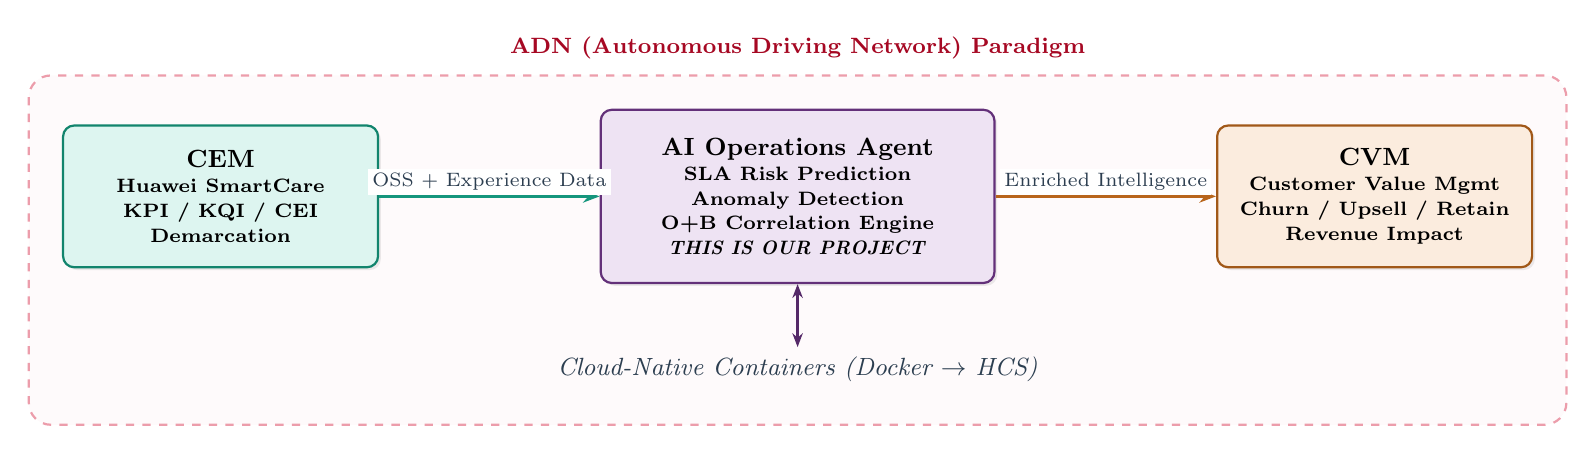
\begin{tikzpicture}[node distance=2.8cm]
  % Nodes
  \node[service=cemteal, minimum width=4cm, minimum height=1.8cm] (cem) {
    \textbf{CEM}\\[-2pt]
    {\scriptsize Huawei SmartCare}\\[-2pt]
    {\scriptsize KPI / KQI / CEI}\\[-2pt]
    {\scriptsize Demarcation}
  };
  
  \node[service=aiviolet, minimum width=5cm, minimum height=2.2cm, right=of cem] (agent) {
    \textbf{AI Operations Agent}\\[-2pt]
    {\scriptsize SLA Risk Prediction}\\[-2pt]
    {\scriptsize Anomaly Detection}\\[-2pt]
    {\scriptsize O+B Correlation Engine}\\[-2pt]
    {\scriptsize \textit{THIS IS OUR PROJECT}}
  };
  
  \node[service=cvmorange, minimum width=4cm, minimum height=1.8cm, right=of agent] (cvm) {
    \textbf{CVM}\\[-2pt]
    {\scriptsize Customer Value Mgmt}\\[-2pt]
    {\scriptsize Churn / Upsell / Retain}\\[-2pt]
    {\scriptsize Revenue Impact}
  };
  
  % Cloud-native label below agent
  \node[below=0.8cm of agent, font=\small\itshape, text=darkbg] (cloud) {
    Cloud-Native Containers (Docker $\to$ HCS)
  };
  
  % Arrows
  \draw[myarrow=cemteal!80!black, line width=1.2pt] (cem) -- (agent)
    node[arrlabel, midway, above] {OSS + Experience Data};
  \draw[myarrow=cvmorange!80!black, line width=1.2pt] (agent) -- (cvm)
    node[arrlabel, midway, above] {Enriched Intelligence};
  \draw[biarrow=aiviolet!60!black, line width=1pt] (agent) -- (cloud);
  
  % Surrounding dashed box
  \begin{scope}[on background layer]
    \node[fit=(cem)(agent)(cvm)(cloud), inner sep=12pt,
          draw=huaweired!40, dashed, rounded corners=8pt,
          fill=huaweired!2, line width=0.8pt] (adn) {};
  \end{scope}
  \node[above=2pt of adn.north, font=\footnotesize\bfseries, text=huaweired!80!black] {
    ADN (Autonomous Driving Network) Paradigm
  };
\end{tikzpicture}
\caption{Industrial positioning: the AI Operations Agent as the intelligence layer between CEM and CVM, within the ADN paradigm.}
\label{fig:cem-agent-cvm}
\end{figure}

The supervisor at Huawei Tunisia validated this positioning: the project implements the exact architectural pattern that Huawei deploys at operator sites, where CEM produces experience signals and CVM consumes business decisions. Our AI Agent is the ``brain'' in the middle, built cloud-natively and portable to Huawei Cloud Stack.

\section{Key Differentiators}

This project distinguishes itself from typical academic proofs-of-concept through three fundamental strengths:

\begin{enumerate}[label=\textbf{\arabic*.}]
  \item \textbf{Real Operator Data:} The models are trained on anonymised production OSS/BSS data from Tunisie Telecom, obtained through the Huawei partnership. This is not synthetic data --- the patterns are real, the anomalies are genuine, and the evaluation metrics are credible. Very few PFE projects at any university have access to real operator data at this scale.
  
  \item \textbf{Cloud-Native Architecture Portable to HCS:} The platform runs as five containerised microservices (Docker Compose) with a clear mapping to Huawei Cloud Stack: MinIO $\to$ OBS, PostgreSQL $\to$ RDS, application services $\to$ ECS/CCE. This is not a theoretical mapping --- the containers are designed from the start for cloud portability.
  
  \item \textbf{AI Agent Bridging CEM and CVM:} The system implements the O+B (OSS+BSS) convergence that is central to Huawei's ADN strategy. It reads SmartCare CEM outputs, correlates them with BSS metrics, and produces actionable CVM inputs. This positions the project squarely within Huawei's industrial roadmap.
\end{enumerate}

\section{Report Structure}

This report is organised as follows:

\begin{itemize}
  \item \textbf{Chapter~\ref{ch:context}} presents the host organisation (Huawei Tunisia), the industrial context of CEM/CVM systems, and the ADN paradigm.
  \item \textbf{Chapter~\ref{ch:stateofart}} surveys the state of the art in AI-driven telecom operations, anomaly detection, and OSS--BSS convergence.
  \item \textbf{Chapter~\ref{ch:architecture}} details the system architecture: the five-service containerised stack, the data lake, the API layer, and the HCS mapping.
  \item \textbf{Chapter~\ref{ch:data}} describes the data strategy: real data ingestion from Tunisie Telecom, the anonymisation pipeline, schema mapping, and the three-layer lake.
  \item \textbf{Chapter~\ref{ch:ai}} documents the AI models: SLA risk prediction, OSS anomaly detection, BSS revenue anomaly detection, and the correlation engine.
  \item \textbf{Chapter~\ref{ch:implementation}} covers the implementation: service code, Docker Compose orchestration, database schema, and the 5-phase pipeline.
  \item \textbf{Chapter~\ref{ch:evaluation}} presents the evaluation results: model metrics (precision, recall, F1), correlation findings, and end-to-end validation.
  \item \textbf{Chapter~\ref{ch:cloud}} describes the cloud deployment strategy and the HCS mapping.
  \item \textbf{Chapter~\ref{ch:conclusion}} concludes the report with a summary, limitations, and future work.
\end{itemize}

% ============================================================================
%  Chapter 2 --- Context: Host Organisation, Industrial Context, ADN
% ============================================================================
\chapter{Project Context}
\label{ch:context}

\section{Host Organisation: Huawei Tunisia}

Huawei Technologies Co., Ltd. is a global leader in information and communications technology (ICT) infrastructure and smart devices. Founded in 1987 in Shenzhen, China, Huawei serves over three billion people worldwide and operates in more than 170 countries. In the telecommunications domain, Huawei provides end-to-end solutions spanning radio access networks (RAN), core networks, transport, and cloud infrastructure.

\textbf{Huawei Tunisia} operates as a regional entity within the North Africa \& Mediterranean business unit. The Cloud IT / Sales-Solution department --- the host of this internship --- focuses on positioning Huawei Cloud Stack (HCS) and associated AI/analytics solutions for Tunisian operators, principally Tunisie Telecom. The team bridges the gap between Huawei's global product portfolio (SmartCare, ADN, HCS) and the specific operational needs of the local market.

This project was conducted within this department, under the direct supervision of the Huawei Cloud IT team, with access to both Huawei's technical documentation and real production data from Tunisie Telecom.

\section{Tunisie Telecom: The Operator Context}

Tunisie Telecom (TT) is the incumbent telecommunications operator in Tunisia, providing fixed and mobile services to millions of subscribers. The Tunisian mobile market is characterised by:

\begin{itemize}
  \item A \textbf{prepaid-dominant} subscriber base ($\sim$80\% prepaid, $\sim$20\% postpaid), consistent with INTT 2023 market statistics;
  \item Three major operators: Tunisie Telecom, Ooredoo Tunisia, and Orange Tunisia;
  \item A growing 4G/LTE footprint with early 5G planning;
  \item Subscriber ARPU (Average Revenue Per User) in the range of 5--105 TND/month, reflecting a wide spectrum from low-recharge prepaid users to premium postpaid subscribers.
\end{itemize}

The data used in this project originates from TT's production environment, anonymised and provided through the Huawei partnership. This real-world grounding is a critical differentiator of the project.

\section{The Telecom OSS/BSS Landscape}

\subsection{Operations Support Systems (OSS)}

OSS encompasses all systems that manage the \emph{network} side of a telecommunications operator. Within Huawei's ecosystem, the OSS layer includes:

\begin{itemize}
  \item \textbf{Access:} RAN (Radio Access Network), FTTx (Fibre to the x), IP access
  \item \textbf{NOM:} Network Operations Management --- fault management, performance management, configuration
  \item \textbf{Core:} Core network elements including IoT platforms
  \item \textbf{Cloud:} Cloud infrastructure management
  \item \textbf{VAS:} Value Added Services management
\end{itemize}

OSS data manifests as KPIs measured per cell, per time window: throughput (Mbps), latency (ms), packet loss (\%), active user count, signal strength (RSRP in dBm), and hundreds of derived indicators.

\subsection{Business Support Systems (BSS)}

BSS encompasses all systems that manage the \emph{business} side: subscriber management, billing, revenue assurance, customer care. Within the context defined by the supervisor, the key BSS metrics include:

\begin{itemize}
  \item \textbf{Norm User:} Standard subscriber behavioural metrics (usage patterns, plan type, line type)
  \item \textbf{EAP:} Experience Analytics Platform --- experience-weighted analytics per subscriber
  \item \textbf{APPU:} Average Purchase Per User --- revenue per recharge or transaction event (TND)
  \item \textbf{DOU:} Data of Use --- monthly data consumption per subscriber (GB)
\end{itemize}

\subsection{The O+B Convergence Challenge: From Scattered Data to Unified Intelligence}

The fundamental challenge in modern telecom operations is \textbf{O+B Convergence}: the unification of OSS and BSS data to move beyond surface-level network analysis. As illustrated in Huawei's unified data architecture framework, the current state of many operators, including TT, is typically characterised by scattered data silos.

In this ``Now'' state, data is split across traditional, separate data warehouses for BSS, OSS, and B2B services. This fragmentation results in complex integration overhead and delayed analytics, ultimately creating an ``AI Blindness'' bottleneck. In this environment, AI initiatives remain stagnant, limited to task-specific chatbots or localized network optimizations that cannot see the broader business impact.

Our project directly implements Huawei's prescribed ``ToBe'' vision: transforming scattered data into centralized, AI-ready intelligence. By substituting siloed warehouses with a unified, three-layer data lake (raw, processed, curated), we establish the foundation for O+B convergence. This centralized data strategy eliminates the delay in analytics and powers an \emph{AI Development Platform} capable of answering complex, cross-domain questions autonomously:

\begin{quote}
\emph{``When cell X degrades, which subscribers are affected, what is the revenue impact, and what retention action should the CVM system trigger?''}
\end{quote}

Today, this question requires manual analysis across multiple systems. Our project automates this correlation, turning scattered AI experiments into scaled, unified productivity.

% ── Figure: Huawei NMS/OSS/BSS Stack ─────────────────────────────────────────
\begin{figure}[H]
\centering
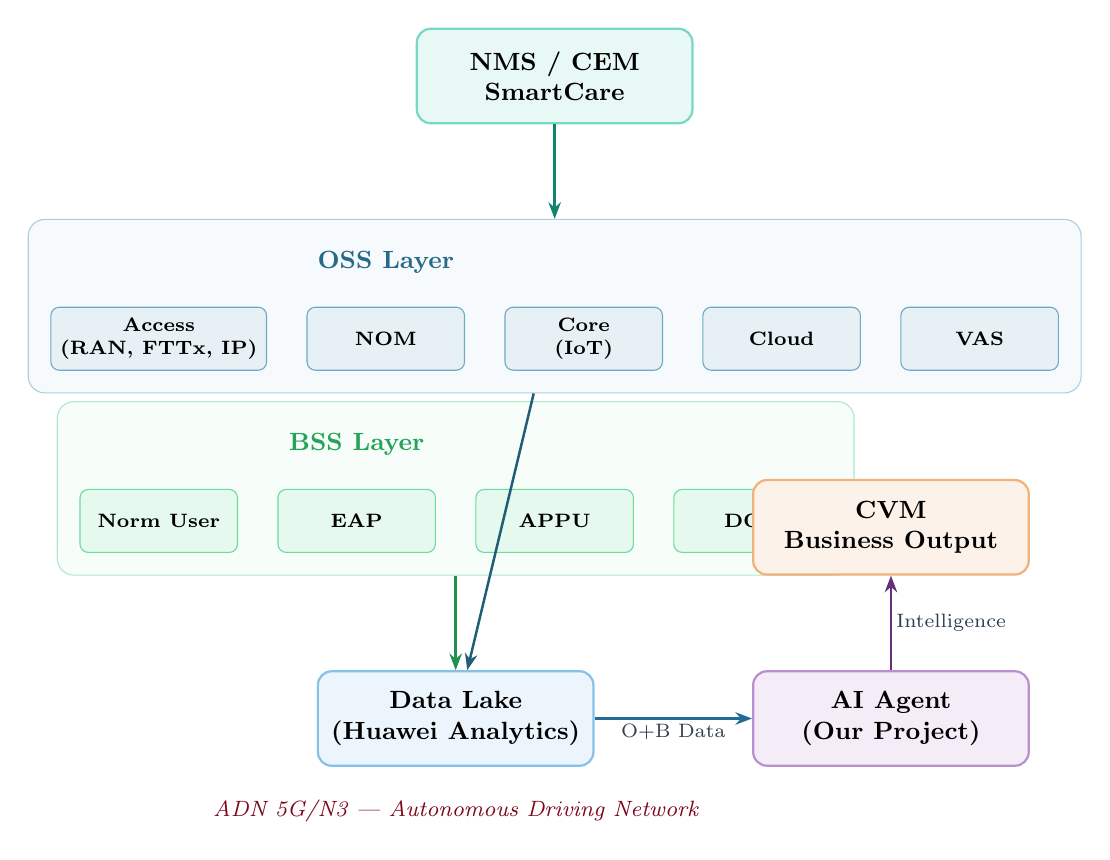
\begin{tikzpicture}[
  node distance=0.4cm and 0.5cm,
  ossbox/.style={rectangle, rounded corners=3pt, minimum width=2cm, minimum height=0.8cm,
    draw=ossblue!70, fill=ossblue!12, font=\scriptsize\bfseries, align=center},
  bssbox/.style={rectangle, rounded corners=3pt, minimum width=2cm, minimum height=0.8cm,
    draw=bssgreen!70, fill=bssgreen!12, font=\scriptsize\bfseries, align=center},
  bigbox/.style={rectangle, rounded corners=5pt, minimum width=3.5cm, minimum height=1.2cm,
    draw=#1!60, fill=#1!10, font=\small\bfseries, align=center, line width=0.8pt},
]

  % OSS Layer
  \node[ossbox] (access) {Access\\(RAN, FTTx, IP)};
  \node[ossbox, right=of access] (nom) {NOM};
  \node[ossbox, right=of nom] (core) {Core\\(IoT)};
  \node[ossbox, right=of core] (cloud) {Cloud};
  \node[ossbox, right=of cloud] (vas) {VAS};
  
  % OSS label
  \node[above=0.3cm of nom, font=\small\bfseries, text=ossblue!80!black] (osslabel) {OSS Layer};
  
  \begin{scope}[on background layer]
    \node[fit=(access)(nom)(core)(cloud)(vas)(osslabel),
          draw=ossblue!40, fill=ossblue!4, rounded corners=6pt, inner sep=8pt] (ossgroup) {};
  \end{scope}

  % BSS Layer --- below
  \node[bssbox, below=1.5cm of access] (normuser) {Norm User};
  \node[bssbox, right=of normuser] (eap) {EAP};
  \node[bssbox, right=of eap] (appu) {APPU};
  \node[bssbox, right=of appu] (dou) {DOU};
  
  \node[above=0.3cm of eap, font=\small\bfseries, text=bssgreen!80!black] (bsslabel) {BSS Layer};
  
  \begin{scope}[on background layer]
    \node[fit=(normuser)(eap)(appu)(dou)(bsslabel),
          draw=bssgreen!40, fill=bssgreen!4, rounded corners=6pt, inner sep=8pt] (bssgroup) {};
  \end{scope}

  % NMS / CEM
  \node[bigbox=cemteal, above=1.2cm of ossgroup] (nms) {\textbf{NMS / CEM}\\SmartCare};
  
  % Data Lake
  \node[bigbox=datalake, below=1.2cm of bssgroup] (lake) {\textbf{Data Lake}\\(Huawei Analytics)};
  
  % AI Agent
  \node[bigbox=aiviolet, right=2cm of lake] (agent) {\textbf{AI Agent}\\(Our Project)};
  
  % CVM
  \node[bigbox=cvmorange, above=1.2cm of agent] (cvm) {\textbf{CVM}\\Business Output};

  % Arrows
  \draw[myarrow=cemteal!70!black] (nms) -- (ossgroup);
  \draw[myarrow=ossblue!70!black] (ossgroup) -- (lake);
  \draw[myarrow=bssgreen!70!black] (bssgroup) -- (lake);
  \draw[myarrow=datalake!70!black] (lake) -- (agent)
    node[arrlabel, midway, below] {O+B Data};
  \draw[myarrow=aiviolet!70!black] (agent) -- (cvm)
    node[arrlabel, midway, right] {Intelligence};
  
  % ADN label
  \node[below=0.3cm of lake, font=\footnotesize\itshape, text=huaweired!60!black] {
    ADN 5G/N3 --- Autonomous Driving Network
  };
  
\end{tikzpicture}
\caption{Huawei NMS/CEM/OSS/BSS ecosystem with data lake and AI Agent positioning (from supervisor notes).}
\label{fig:huawei-stack}
\end{figure}

\section{Customer Experience Management (CEM) and SmartCare}

Huawei SmartCare is a CEM platform deployed at operator sites worldwide. Its core functions include:

\begin{itemize}
  \item \textbf{KPI/KQI/CEI Computation:} From raw network counters, SmartCare derives Key Quality Indicators (KQI) and Customer Experience Indices (CEI) per subscriber, per service, per cell.
  \item \textbf{Demarcation:} When a service degrades, SmartCare identifies \emph{where} the problem is --- in the RAN, the core, the transport, or the service platform. This is the ``demarcation function.''
  \item \textbf{Experience Alerts:} Real-time alerts when a subscriber's experience drops below configurable thresholds.
\end{itemize}

Our platform maps directly to SmartCare's output:
\begin{itemize}
  \item Our \emph{SLA risk prediction} corresponds to SmartCare's experience risk scoring.
  \item Our \emph{anomaly detection} corresponds to SmartCare's demarcation function --- identifying abnormal cells and subscribers.
  \item Our \emph{OSS--BSS correlation engine} extends SmartCare's reach by linking experience degradation to revenue impact --- a function SmartCare itself does not perform.
\end{itemize}

\section{Customer Value Management (CVM) and the AI Intelligence Gap}

CVM systems consume intelligence about subscribers to drive business actions. However, without a unified data foundation bridging CEM and business data, the integration remains complex and reactive. A mature CVM demands:

\begin{itemize}
  \item \textbf{Churn prediction:} Identifying at-risk subscribers before they leave due to invisible network degradation.
  \item \textbf{Upsell triggers:} Recommending higher-tier plans to highly engaged users consuming large volumes of data (DoU).
  \item \textbf{Retention actions:} Proactive offers (bonus data, discounts) automatically targeted at subscribers experiencing documented service drops (SLA risks).
  \item \textbf{Revenue impact scoring:} Quantifying the exact business cost (via APPU and Revenue) of network anomalies.
\end{itemize}

As positioned in Huawei's target architecture, the consumers of a unified AI platform include AI assistants, marketing copilots, and intelligent network analysts. Our AI Agent fills this specific gap---the intelligence layer bridging CEM outputs to CVM inputs. It produces exactly the required intelligent triggers: churn-correlated anomaly flags, SLA risk scores, and revenue impact assessments, natively exposing these cross-domain insights via REST API for immediate business action.

\section{The Autonomous Driving Network (ADN) Paradigm: Achieving L4 Autonomy}

Huawei's ADN vision charts the evolution of telecom networks through progressive levels of autonomy, mirroring the automotive industry. Recently updated industry frameworks recognize the progression of AI intelligence from basic Chatbots (L1) and Reasoners (L2) to fully autonomous, complex organizations (L5). 

\begin{itemize}
  \item \textbf{L1 --- Assisted (Chatbot):} Able to answer basic questions; manual operations with simple tool support.
  \item \textbf{L2 --- Partial (Reasoner):} Able to think; some automated, human-supervised workflows.
  \item \textbf{L3 --- Conditional (Agent):} \emph{Able to do}. The era of AI Agents taking automated actions under human supervision.
  \item \textbf{L4 --- Highly Autonomous (Innovator):} \emph{Able to invent and decide}. AI manages complex workflows and executes automated remediation without human intervention.
  \item \textbf{L5 --- Fully Autonomous (Organization):} Able to manage large and complex systems; the network manages itself end-to-end.
\end{itemize}

Historically, network analytics have been stuck in passive analytics (L1/L2) or conditional alerts (L3). Our project is explicitly designed to pierce the \textbf{L4 (Highly Autonomous)} threshold. It achieves this by moving beyond merely generating dashboards. The pipeline acts as an autonomous intelligence engine that actively ingests O+B data, orchestrates parallel ML models (Gradient Boosting, Isolation Forests), and critically, \textbf{generates and pushes autonomous action triggers} (e.g., CVM retention payloads, automated SLA breach escalations) without human intervention. By proving that the agent can "decide and act" to prevent revenue loss, this project serves as a foundational L4 proof-of-concept for the ultimate L5 Huawei vision.

% ── Figure: ADN Levels ────────────────────────────────────────────────────────
\begin{figure}[H]
\centering
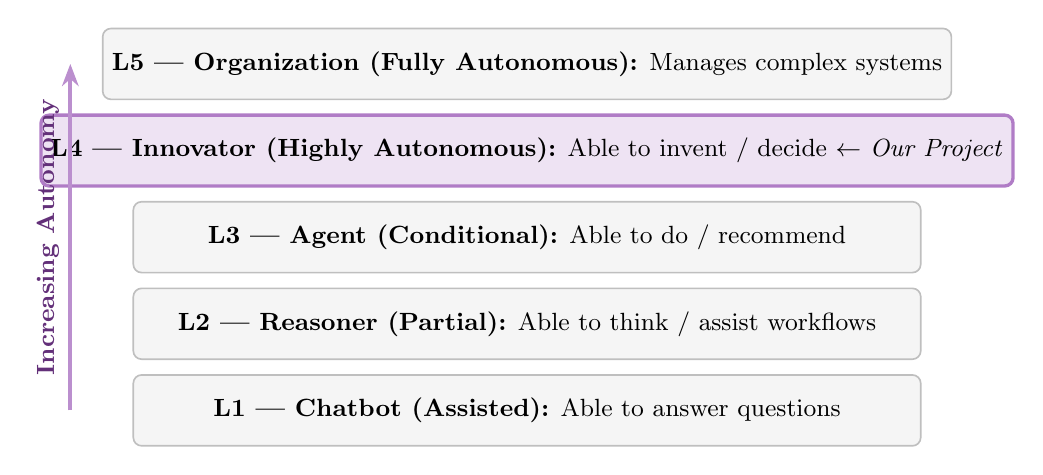
\begin{tikzpicture}[
  level/.style={
    rectangle, rounded corners=3pt, minimum width=10cm, minimum height=0.9cm,
    font=\small, align=center, line width=0.6pt,
  },
]
  \node[level, draw=gray!50, fill=gray!8] (l1) at (0,0)
    {\textbf{L1 --- Chatbot (Assisted):} Able to answer questions};
  \node[level, draw=gray!50, fill=gray!8] (l2) at (0,1.1)
    {\textbf{L2 --- Reasoner (Partial):} Able to think / assist workflows};
  \node[level, draw=gray!50, fill=gray!8] (l3) at (0,2.2)
    {\textbf{L3 --- Agent (Conditional):} Able to do / recommend};
  \node[level, draw=aiviolet!70, fill=aiviolet!15, line width=1.2pt] (l4) at (0,3.3)
    {\textbf{L4 --- Innovator (Highly Autonomous):} Able to invent / decide $\leftarrow$ \textit{Our Project}};
  \node[level, draw=gray!50, fill=gray!8] (l5) at (0,4.4)
    {\textbf{L5 --- Organization (Fully Autonomous):} Manages complex systems};
  
  % Arrow on the side
  \draw[-{Stealth[length=8pt]}, line width=1.5pt, aiviolet!60] (-5.8,0) -- (-5.8,4.4)
    node[midway, rotate=90, above, font=\small\bfseries, text=aiviolet!70!black] {Increasing Autonomy};
\end{tikzpicture}
\caption{Huawei ADN autonomy levels. Our project targets L4 --- Highly Autonomous.}
\label{fig:adn-levels}
\end{figure}

\section{Project Scope and Boundaries}

\subsection{In Scope}

\begin{itemize}
  \item Ingestion of real anonymised OSS/BSS data from Tunisie Telecom via Huawei
  \item Three-layer data lake: Raw $\to$ Processed $\to$ Curated (MinIO / OBS)
  \item Three ML models: SLA risk (GBR), OSS anomalies (IF), BSS anomalies (IF)
  \item OSS--BSS statistical correlation engine (Pearson/Spearman)
  \item RESTful API for insight consumption
  \item Docker Compose orchestration (5 services)
  \item Architectural mapping to HCS (OBS, RDS, ECS/CCE)
  \item Model evaluation with real data (precision, recall, F1, confusion matrix)
\end{itemize}

\subsection{Explicitly Out of Scope}

\begin{itemize}
  \item Vendor-grade telecom assurance at production scale (millions of subscribers)
  \item Real-time streaming ingestion (our batch pipeline demonstrates the architecture)
  \item Direct SmartCare API integration (we ingest CEM-equivalent data from exports)
  \item Production HCS deployment (architectural readiness, not production cutover)
  \item CVM action execution (the AI Agent produces intelligence; CVM acts on it)
\end{itemize}

\section{Chapter Summary}

This chapter established the industrial context of the project: the Huawei CEM/CVM ecosystem, the SmartCare platform, the O+B convergence challenge, and the ADN paradigm. The project is positioned as the intelligence layer between CEM and CVM, implemented cloud-natively and trained on real Tunisie Telecom data. The next chapter surveys the state of the art in AI-driven telecom operations, positioning our approach relative to existing academic and industrial work.

% ============================================================================
%  Chapter 3 --- State of the Art
% ============================================================================
\chapter{State of the Art}
\label{ch:stateofart}

\section{Introduction}

This chapter surveys the current state of AI-driven telecom operations, anomaly detection techniques, and OSS--BSS convergence approaches. We position our work relative to existing academic and industrial solutions, identifying the gaps that our AI Operations Agent addresses.

\section{AI in Telecommunications Operations}

\subsection{The AIOps Paradigm}

AIOps (Artificial Intelligence for IT Operations) has emerged as the dominant framework for applying machine learning to operational data. Originally coined by Gartner, AIOps platforms ingest telemetry data from multiple sources, apply ML models for anomaly detection, event correlation, and root cause analysis, and produce actionable recommendations.

In the telecom domain, AIOps extends to:
\begin{itemize}
  \item \textbf{Network performance prediction:} Using historical KPI data to forecast SLA breaches before they occur.
  \item \textbf{Anomaly detection:} Identifying abnormal network behaviour from cell-level metrics without explicit labels.
  \item \textbf{Root cause analysis:} Correlating symptoms across multiple network elements to locate the origin of degradation.
  \item \textbf{Self-healing:} Automatic remediation actions triggered by AI decisions (ADN L4/L5).
\end{itemize}

\subsection{Existing Approaches}

Table~\ref{tab:related-work} summarises relevant approaches in the literature.

\begin{table}[H]
\centering
\caption{Comparison of related AI-driven telecom approaches.}
\label{tab:related-work}
\small
\begin{tabularx}{\textwidth}{@{}lXcccc@{}}
\toprule
\textbf{Approach} & \textbf{Focus} & \textbf{Real Data} & \textbf{O+B} & \textbf{Cloud} & \textbf{Agent} \\
\midrule
SELFNET~\cite{selfnet2017} & Self-healing 5G networks & Simulated & No & No & No \\
ETSI ZSM~\cite{etsi_zsm} & Zero-touch management architecture & Spec only & Partial & Yes & Partial \\
Nokia AVA~\cite{nokia_ava} & Telecom analytics platform & Yes & No & Yes & No \\
Huawei SmartCare~\cite{smartcare} & CEM with demarcation & Yes & Partial & Yes & No \\
Ericsson EOM~\cite{ericsson_eom} & Expert-system operations & Yes & No & Yes & No \\
Academic IF-based~\cite{if_telecom} & Anomaly detection on KPIs & Synthetic & No & No & No \\
\textbf{Our Project} & \textbf{CEM--CVM AI Agent} & \textbf{Yes (TT)} & \textbf{Yes} & \textbf{Yes} & \textbf{Yes} \\
\bottomrule
\end{tabularx}
\end{table}

The key observation is that existing solutions either focus on the OSS side (network anomaly detection) or the BSS side (revenue analytics), but rarely bridge both. When they do (SmartCare, ETSI ZSM), the intelligence layer is either manual or limited to rule-based correlation. Our project is unique in combining real data, O+B convergence, cloud-native deployment, and an agentic AI architecture.

\section{Anomaly Detection in Telecom Networks}

\subsection{Supervised vs. Unsupervised Approaches}

Anomaly detection in telecommunications can be approached through supervised or unsupervised methods:

\begin{itemize}
  \item \textbf{Supervised:} Requires labelled data (normal vs. anomalous). Common classifiers include Random Forest, XGBoost, and neural networks. The challenge is obtaining labelled data in production environments --- operators rarely label every anomaly event comprehensively.
  \item \textbf{Unsupervised:} Does not require labels. Methods include Isolation Forest, One-Class SVM, DBSCAN, and autoencoders. These methods learn the ``normal'' distribution and flag deviations.
\end{itemize}

\subsection{Isolation Forest}

Isolation Forest (IF), introduced by Liu et al. (2008), is particularly well-suited to telecom anomaly detection because:

\begin{enumerate}
  \item It operates on numeric tabular data at high speed and low memory.
  \item It does not require labels, which matches the real-world telecom scenario.
  \item It naturally handles high-dimensional feature spaces.
  \item Its ``contamination'' parameter allows domain-informed tuning of anomaly prevalence.
  \item It produces both hard decisions ($\pm 1$) and continuous anomaly scores.
\end{enumerate}

IF constructs an ensemble of random trees. Each tree recursively selects a random feature and a random split value. Anomalies --- being ``few and different'' --- require fewer splits to be isolated, resulting in shorter path lengths. The anomaly score is derived from the average path length across all trees.

\subsection{Gradient Boosting for Risk Prediction}

For supervised regression tasks such as SLA risk prediction, Gradient Boosting Regressors (GBR) are the method of choice for tabular telecom data. GBR builds an ensemble of weak learners (shallow decision trees) sequentially, with each tree correcting the errors of the previous ensemble. Key advantages for our use case:

\begin{itemize}
  \item Handles non-linear KPI interactions (e.g., high latency \emph{and} packet loss amplifies risk more than either alone).
  \item Provides feature importances for explainability --- critical during the PFE defence.
  \item Strong performance on small-to-medium tabular datasets (our data scale).
  \item Well-understood, academically defensible, and supported by scikit-learn.
\end{itemize}

\section{OSS--BSS Convergence}

\subsection{The Convergence Problem}

OSS and BSS data have historically been managed by separate teams, stored in separate systems, and analysed with separate tools. The TM Forum's ODA (Open Digital Architecture) initiative explicitly identifies OSS--BSS convergence as a strategic priority. Huawei's O+B convergence vision aligns with this broader industry movement.

\subsection{Statistical Correlation Methods}

We employ two complementary correlation methods:

\begin{itemize}
  \item \textbf{Pearson correlation:} Measures the \emph{linear} relationship between two variables. A Pearson coefficient of $r = -0.8$ between latency and revenue would indicate that as latency increases, revenue decreases linearly.
  \item \textbf{Spearman correlation:} Measures the \emph{monotonic} (rank-based) relationship. It captures non-linear but consistent trends --- for example, revenue tends to decrease when packet loss increases, even if the relationship is not strictly linear.
\end{itemize}

By computing both Pearson and Spearman on multiple OSS--BSS metric pairs, we produce a comprehensive picture of how network degradation manifests in business outcomes.

\section{Cloud-Native Architecture in Telecom}

\subsection{The Shift to Cloud-Native}

The telecom industry is undergoing a fundamental architectural shift from monolithic network functions to cloud-native, containerised microservices. This shift is driven by:

\begin{itemize}
  \item \textbf{ETSI NFV:} Network Functions Virtualisation decouples software from hardware.
  \item \textbf{5G SBA:} 5G's Service-Based Architecture defines network functions as loosely coupled services.
  \item \textbf{Kubernetes / Docker:} Container orchestration enables horizontal scaling, rolling updates, and infrastructure abstraction.
\end{itemize}

\subsection{Huawei Cloud Stack (HCS)}

Huawei Cloud Stack is Huawei's hybrid cloud platform, deployed on-premises at operator sites. It provides:

\begin{itemize}
  \item \textbf{OBS (Object Storage Service):} S3-compatible object storage --- equivalent to our MinIO.
  \item \textbf{RDS (Relational Database Service):} Managed PostgreSQL/MySQL --- equivalent to our PostgreSQL container.
  \item \textbf{ECS/CCE:} Elastic Cloud Server / Cloud Container Engine --- container runtime equivalent to our Docker Compose.
  \item \textbf{VPC:} Network isolation and security boundaries.
\end{itemize}

Our architecture is designed from inception for HCS portability: the same Docker containers, with environment variable changes, can run on HCS with minimal modification.

\section{Gap Analysis and Positioning}

% ── Figure: Gap Analysis ──────────────────────────────────────────────────────
\begin{figure}[H]
\centering
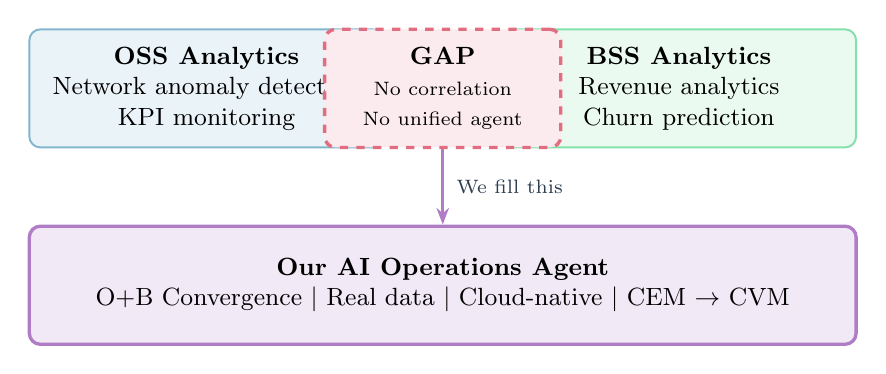
\begin{tikzpicture}[
  gapnode/.style={
    rectangle, rounded corners=4pt, minimum width=4.5cm, minimum height=1.5cm,
    font=\small, align=center, line width=0.7pt,
  },
]
  % Existing solutions
  \node[gapnode, draw=ossblue!60, fill=ossblue!10] (oss) at (0,0) {
    \textbf{OSS Analytics}\\
    Network anomaly detection\\
    KPI monitoring
  };
  \node[gapnode, draw=bssgreen!60, fill=bssgreen!10] (bss) at (6,0) {
    \textbf{BSS Analytics}\\
    Revenue analytics\\
    Churn prediction
  };
  
  % Gap
  \node[gapnode, draw=huaweired!60, fill=huaweired!8,
        minimum width=3cm, minimum height=1.5cm,
        dashed, line width=1.2pt] (gap) at (3,0) {
    \textbf{GAP}\\
    \scriptsize No correlation\\
    \scriptsize No unified agent
  };
  
  % Our solution
  \node[gapnode, draw=aiviolet!70, fill=aiviolet!12,
        minimum width=10.5cm, minimum height=1.5cm,
        line width=1.2pt] (ours) at (3,-2.5) {
    \textbf{Our AI Operations Agent}\\
    O+B Convergence $|$ Real data $|$ Cloud-native $|$ CEM $\to$ CVM
  };
  
  % Arrows
  \draw[myarrow=aiviolet!70, line width=1pt] (gap) -- (ours)
    node[arrlabel, midway, right, xshift=3pt] {We fill this};
    
\end{tikzpicture}
\caption{Gap analysis: our AI Operations Agent bridges the OSS--BSS analytics gap.}
\label{fig:gap-analysis}
\end{figure}

The state of the art leaves a clear architectural gap: no existing PFE-scale solution combines real operator data, O+B convergence, cloud-native deployment, and an agentic AI architecture that bridges CEM and CVM. Our project fills this gap.

\section{Chapter Summary}

This chapter surveyed AI in telecom operations, anomaly detection methods (Isolation Forest, Gradient Boosting), OSS--BSS convergence challenges, and cloud-native telecom architectures. We identified the gap between existing CEM and CVM platforms --- the absence of a unified AI intelligence layer --- and positioned our project as the solution. The next chapter details the system architecture.

% ============================================================================
%  Chapter 4 --- System Architecture
% ============================================================================
\chapter{System Architecture}
\label{ch:architecture}

\section{Introduction}

This chapter presents the architecture of the AI Operations Agent platform. We describe the system at four levels of abstraction: the high-level CEM--CVM positioning (Section~\ref{sec:arch-highlevel}), the container-level service decomposition (Section~\ref{sec:arch-containers}), the data flow through the pipeline (Section~\ref{sec:arch-pipeline}), and the data lake architecture (Section~\ref{sec:arch-datalake}).

\section{High-Level Architecture: CEM $\to$ AI Agent $\to$ CVM}
\label{sec:arch-highlevel}

At the highest level, the system is the intelligence bridge between two Huawei ecosystem components:

\begin{itemize}
  \item \textbf{Upstream (CEM/SmartCare):} Provides KPI/KQI/CEI scores, demarcation results, and experience alerts. In our implementation, this data arrives as real OSS exports from Tunisie Telecom (CSV/Excel/JSON files).
  \item \textbf{Downstream (CVM):} Consumes churn predictions, SLA risk scores, anomaly alerts, upsell triggers, and revenue impact correlations. In our implementation, CVM reads these from our REST API.
\end{itemize}

The AI Agent sits in the middle and performs four core functions:
\begin{enumerate}
  \item \textbf{Ingestion:} Reads OSS and BSS data, anonymises sensitive fields, maps to the internal schema.
  \item \textbf{Analysis:} Runs ML inference --- SLA risk scoring, network anomaly detection, revenue anomaly detection.
  \item \textbf{Correlation:} Computes statistical correlations between OSS degradation and BSS impact.
  \item \textbf{Serving:} Exposes all results through REST endpoints, persists to a serving database.
\end{enumerate}

\section{Container Architecture}
\label{sec:arch-containers}

The platform is decomposed into five containerised microservices, orchestrated by Docker Compose.

% ── Figure: Container Architecture ────────────────────────────────────────────
\begin{figure}[H]
\centering
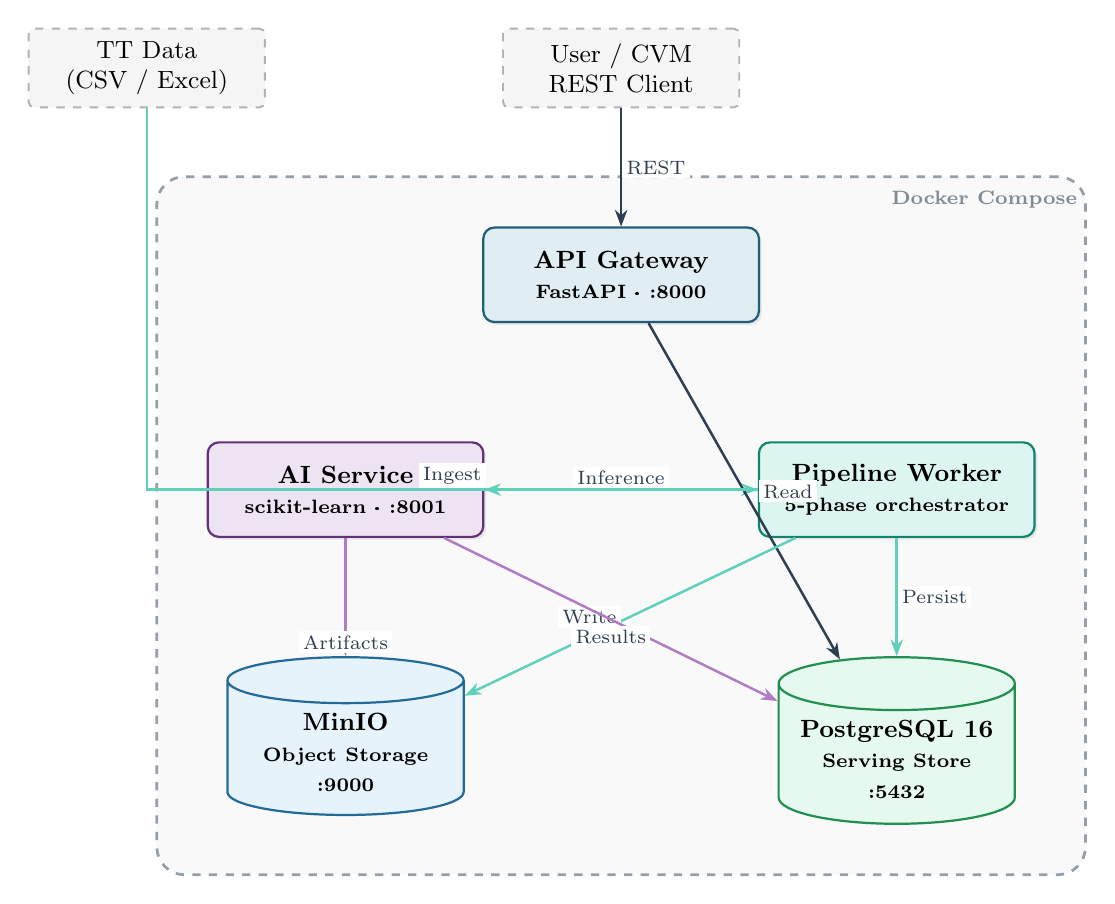
\begin{tikzpicture}[node distance=1.5cm and 2cm]

  % External
  \node[external, minimum width=3cm] (user) {User / CVM\\REST Client};
  \node[external, minimum width=3cm, left=3cm of user] (ttdata) {TT Data\\(CSV / Excel)};
  
  % Services
  \node[service=ossblue, below=1.5cm of user, minimum width=3.5cm] (apigw) {
    \textbf{API Gateway}\\{\scriptsize FastAPI · :8000}
  };
  
  \node[service=aiviolet, below=of apigw, minimum width=3.5cm, xshift=-3.5cm] (ai) {
    \textbf{AI Service}\\{\scriptsize scikit-learn · :8001}
  };
  
  \node[service=cemteal, below=of apigw, minimum width=3.5cm, xshift=3.5cm] (worker) {
    \textbf{Pipeline Worker}\\{\scriptsize 5-phase orchestrator}
  };
  
  \node[datastore=datalake, below=1.5cm of ai, minimum width=3cm] (minio) {
    \textbf{MinIO}\\{\scriptsize Object Storage}\\{\scriptsize :9000}
  };
  
  \node[datastore=bssgreen, below=1.5cm of worker, minimum width=3cm] (pg) {
    \textbf{PostgreSQL 16}\\{\scriptsize Serving Store}\\{\scriptsize :5432}
  };
  
  % Docker boundary
  \begin{scope}[on background layer]
    \node[fit=(apigw)(ai)(worker)(minio)(pg),
          draw=darkbg!50, fill=darkbg!3, rounded corners=10pt,
          inner sep=18pt, line width=1pt, dashed] (docker) {};
  \end{scope}
  \node[below=2pt of docker.north east, anchor=north east,
        font=\scriptsize\bfseries, text=darkbg!60] {Docker Compose};
  
  % Arrows
  \draw[myarrow] (user) -- (apigw) node[arrlabel, midway, right] {REST};
  \draw[myarrow=cemteal!70] (ttdata) |- (worker) node[arrlabel, pos=0.75, above] {Ingest};
  
  \draw[myarrow] (apigw) -- (pg) node[arrlabel, midway, right, xshift=5pt] {Read};
  \draw[myarrow=cemteal!70] (worker) -- (ai) node[arrlabel, midway, above] {Inference};
  \draw[myarrow=cemteal!70] (worker) -- (minio) node[arrlabel, midway, left, xshift=-3pt] {Write};
  \draw[myarrow=cemteal!70] (worker) -- (pg) node[arrlabel, midway, right] {Persist};
  \draw[myarrow=aiviolet!70] (ai) -- (pg) node[arrlabel, midway, below, yshift=-2pt] {Results};
  \draw[myarrow=aiviolet!70] (ai) -- (minio) node[arrlabel, midway, below, yshift=-12pt] {Artifacts};
  
\end{tikzpicture}
\caption{Container-level architecture: five services orchestrated by Docker Compose.}
\label{fig:container-arch}
\end{figure}

\subsection{Service Descriptions}

\begin{table}[H]
\centering
\caption{Service inventory and responsibilities.}
\label{tab:services}
\begin{tabularx}{\textwidth}{@{}lllX@{}}
\toprule
\textbf{Service} & \textbf{Technology} & \textbf{Port} & \textbf{Responsibility} \\
\midrule
API Gateway  & FastAPI (Python)   & 8000 & REST endpoint serving: SLA risk, anomalies, correlations, revenue anomalies, pipeline runs \\
AI Service   & scikit-learn + FastAPI & 8001 & ML model hosting (GBR + IF $\times 2$), model training on startup, inference via POST \\
Pipeline Worker & Python (run-once) & --- & 5-phase orchestration: data ingestion, feature engineering, inference, decision \& action, curation \\
PostgreSQL 16 & Official image    & 5432 & Serving store with 8 tables: pipeline runs, datasets, models, anomalies, SLA risk, correlations, revenue anomalies, action recommendations \\
MinIO        & Official image     & 9000 & S3-compatible object storage: 3-layer data lake (raw/processed/curated) \\
\bottomrule
\end{tabularx}
\end{table}

\subsection{Inter-Service Communication}

All communication between services uses synchronous HTTP REST calls over the Docker internal network. The pipeline worker is the primary orchestrator --- it drives the entire data flow by calling the AI service for inference and writing results to both MinIO and PostgreSQL.

\section{Pipeline Architecture}
\label{sec:arch-pipeline}

The pipeline worker executes a 5-phase workflow that transforms raw data into actionable intelligence and autonomous recommendations.

% ── Figure: Pipeline Sequence ─────────────────────────────────────────────────
\begin{figure}[H]
\centering
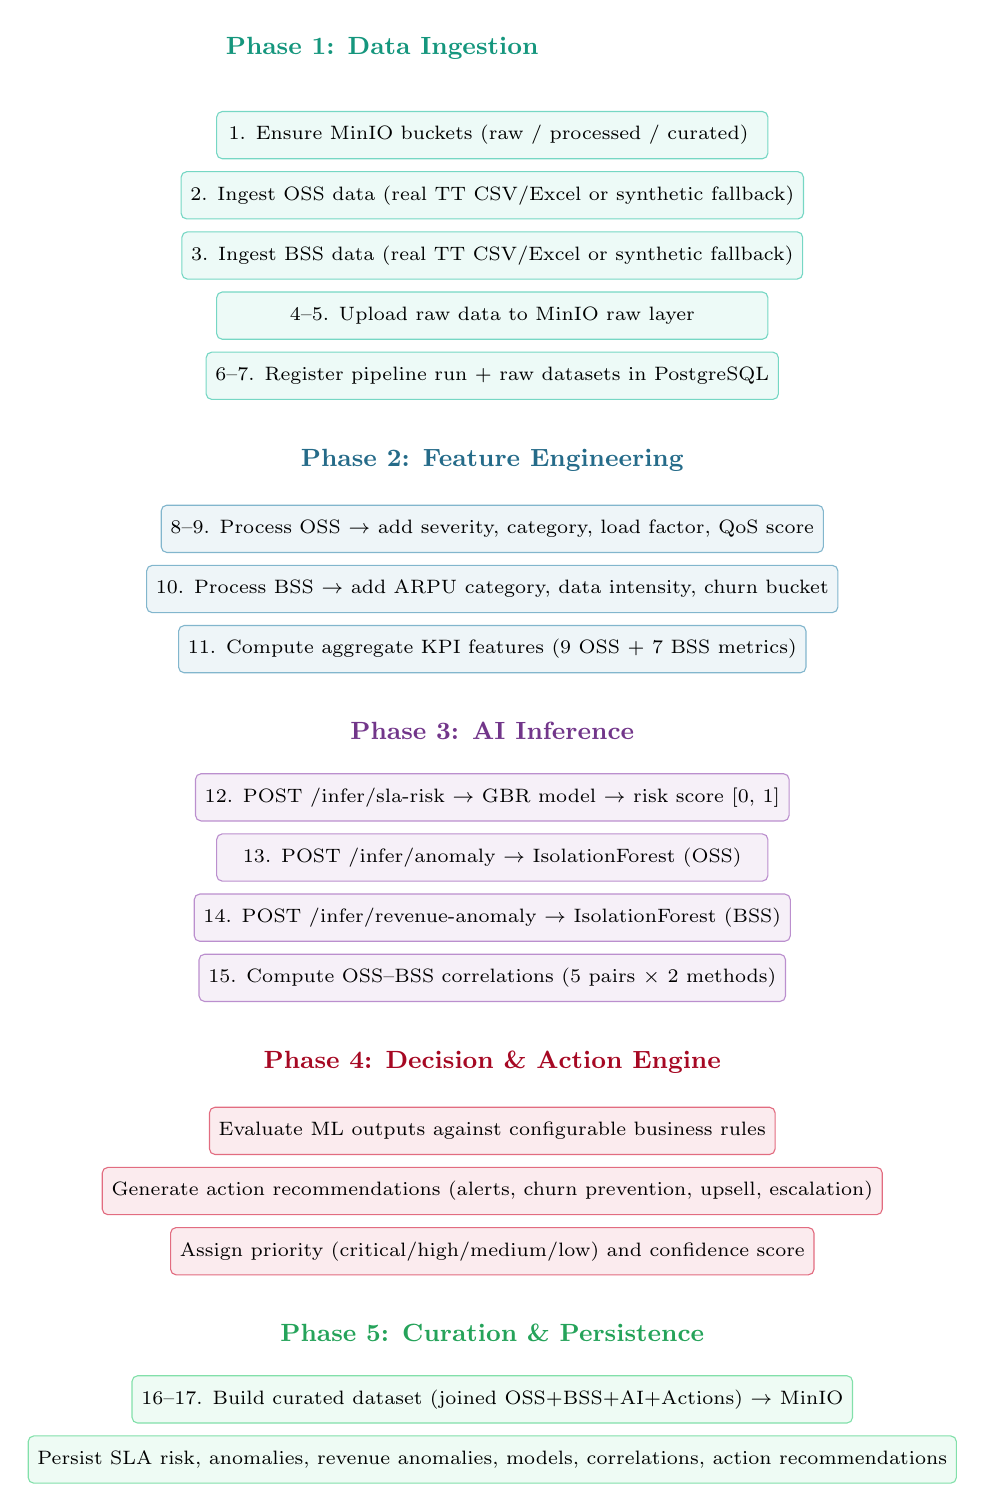
\begin{tikzpicture}[
  step/.style={
    rectangle, rounded corners=2pt, minimum width=7cm, minimum height=0.6cm,
    draw=#1!60, fill=#1!8, font=\scriptsize, align=left, text=black,
  },
  phase/.style={
    font=\small\bfseries, text=#1!80!black, anchor=west,
  },
  node distance=0.15cm,
]

  % Phase 1: Ingestion
  \node[phase=cemteal] (p1) at (0,0) {Phase 1: Data Ingestion};
  \node[step=cemteal, below=0.3cm of p1, anchor=north west] (s1) at (0,-0.5) {
    1. Ensure MinIO buckets (raw / processed / curated)
  };
  \node[step=cemteal, below=of s1] (s2) {2. Ingest OSS data (real TT CSV/Excel or synthetic fallback)};
  \node[step=cemteal, below=of s2] (s3) {3. Ingest BSS data (real TT CSV/Excel or synthetic fallback)};
  \node[step=cemteal, below=of s3] (s4) {4--5. Upload raw data to MinIO raw layer};
  \node[step=cemteal, below=of s4] (s5) {6--7. Register pipeline run + raw datasets in PostgreSQL};
  
  % Phase 2: Processing
  \node[phase=ossblue, below=0.5cm of s5] (p2) {Phase 2: Feature Engineering};
  \node[step=ossblue, below=0.3cm of p2] (s6) {8--9. Process OSS $\to$ add severity, category, load factor, QoS score};
  \node[step=ossblue, below=of s6] (s7) {10. Process BSS $\to$ add ARPU category, data intensity, churn bucket};
  \node[step=ossblue, below=of s7] (s8) {11. Compute aggregate KPI features (9 OSS + 7 BSS metrics)};
  
  % Phase 3: AI Inference
  \node[phase=aiviolet, below=0.5cm of s8] (p3) {Phase 3: AI Inference};
  \node[step=aiviolet, below=0.3cm of p3] (s9) {12. POST /infer/sla-risk $\to$ GBR model $\to$ risk score [0, 1]};
  \node[step=aiviolet, below=of s9] (s10) {13. POST /infer/anomaly $\to$ IsolationForest (OSS)};
  \node[step=aiviolet, below=of s10] (s11) {14. POST /infer/revenue-anomaly $\to$ IsolationForest (BSS)};
  \node[step=aiviolet, below=of s11] (s12) {15. Compute OSS--BSS correlations (5 pairs $\times$ 2 methods)};
  
  % Phase 4: Decision & Action
  \node[phase=huaweired, below=0.5cm of s12] (p4) {Phase 4: Decision \& Action Engine};
  \node[step=huaweired, below=0.3cm of p4] (s13a) {Evaluate ML outputs against configurable business rules};
  \node[step=huaweired, below=of s13a] (s13b) {Generate action recommendations (alerts, churn prevention, upsell, escalation)};
  \node[step=huaweired, below=of s13b] (s13c) {Assign priority (critical/high/medium/low) and confidence score};
  
  % Phase 5: Persistence
  \node[phase=bssgreen, below=0.5cm of s13c] (p5) {Phase 5: Curation \& Persistence};
  \node[step=bssgreen, below=0.3cm of p5] (s14) {16--17. Build curated dataset (joined OSS+BSS+AI+Actions) $\to$ MinIO};
  \node[step=bssgreen, below=of s14] (s15) {Persist SLA risk, anomalies, revenue anomalies, models, correlations, action recommendations};
  
\end{tikzpicture}
\caption{The 5-phase pipeline execution flow.}
\label{fig:pipeline-flow}
\end{figure}

\section{Data Lake Architecture}
\label{sec:arch-datalake}

The platform implements a three-layer data lake using MinIO (locally) or OBS (on HCS):

% ── Figure: Data Lake Layers ──────────────────────────────────────────────────
\begin{figure}[H]
\centering
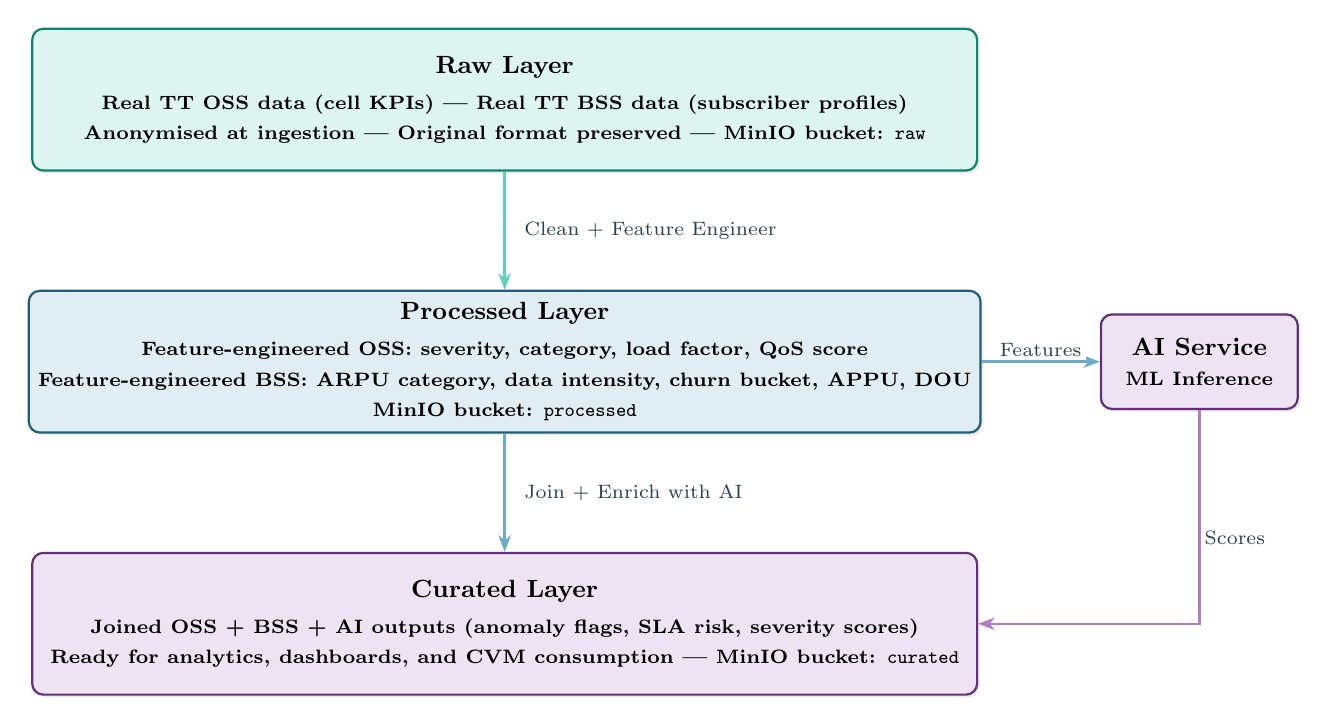
\begin{tikzpicture}[node distance=1.5cm]

  % Raw Layer
  \node[service=cemteal, minimum width=12cm, minimum height=1.8cm] (raw) {
    \textbf{Raw Layer}\\[2pt]
    {\scriptsize Real TT OSS data (cell KPIs) | Real TT BSS data (subscriber profiles)}\\
    {\scriptsize Anonymised at ingestion | Original format preserved | MinIO bucket: \texttt{raw}}
  };
  
  % Processed Layer
  \node[service=ossblue, minimum width=12cm, minimum height=1.8cm, below=of raw] (proc) {
    \textbf{Processed Layer}\\[2pt]
    {\scriptsize Feature-engineered OSS: severity, category, load factor, QoS score}\\
    {\scriptsize Feature-engineered BSS: ARPU category, data intensity, churn bucket, APPU, DOU}\\
    {\scriptsize MinIO bucket: \texttt{processed}}
  };
  
  % Curated Layer
  \node[service=aiviolet, minimum width=12cm, minimum height=1.8cm, below=of proc] (cur) {
    \textbf{Curated Layer}\\[2pt]
    {\scriptsize Joined OSS + BSS + AI outputs (anomaly flags, SLA risk, severity scores)}\\
    {\scriptsize Ready for analytics, dashboards, and CVM consumption | MinIO bucket: \texttt{curated}}
  };
  
  % AI Service on the side
  \node[service=aiviolet, right=1.5cm of proc, minimum width=2.5cm] (aiside) {
    \textbf{AI Service}\\{\scriptsize ML Inference}
  };
  
  % Arrows
  \draw[myarrow=cemteal!70, line width=1.2pt] (raw) -- (proc)
    node[arrlabel, midway, right, xshift=5pt] {Clean + Feature Engineer};
  \draw[myarrow=ossblue!70, line width=1.2pt] (proc) -- (cur)
    node[arrlabel, midway, right, xshift=5pt] {Join + Enrich with AI};
  \draw[myarrow=ossblue!70, line width=0.9pt] (proc) -- (aiside)
    node[arrlabel, midway, above] {Features};
  \draw[myarrow=aiviolet!70, line width=0.9pt] (aiside) |- (cur)
    node[arrlabel, pos=0.3, right] {Scores};
    
\end{tikzpicture}
\caption{Three-layer data lake architecture: Raw $\to$ Processed $\to$ Curated.}
\label{fig:datalake}
\end{figure}

\subsection{Layer Descriptions}

\begin{itemize}
  \item \textbf{Raw Layer:} Contains ingested data as received from Tunisie Telecom, after anonymisation (MSISDN hashing, address stripping). No transformations are applied. Data is stored as JSON/CSV objects in the \texttt{raw} MinIO bucket, preserving the original structure for auditability.
  
  \item \textbf{Processed Layer:} Contains feature-engineered data ready for ML inference. OSS records gain computed fields (latency severity, throughput category, load factor, QoS composite score). BSS records gain ARPU category, data intensity classes, churn risk buckets, and explicit APPU/DOU values. Stored in the \texttt{processed} bucket.
  
  \item \textbf{Curated Layer:} Contains the joined OSS+BSS dataset enriched with AI model outputs: anomaly flags, anomaly scores, SLA risk scores, and correlation insights. This is the ``gold'' layer, ready for dashboard consumption, CVM integration, or further analysis. Stored in the \texttt{curated} bucket.
\end{itemize}

\section{Database Architecture}

PostgreSQL 16 serves as the metadata and serving store. The schema comprises eight tables:

% ── Figure: ER Diagram (TikZ) ─────────────────────────────────────────────────
\begin{figure}[H]
\centering
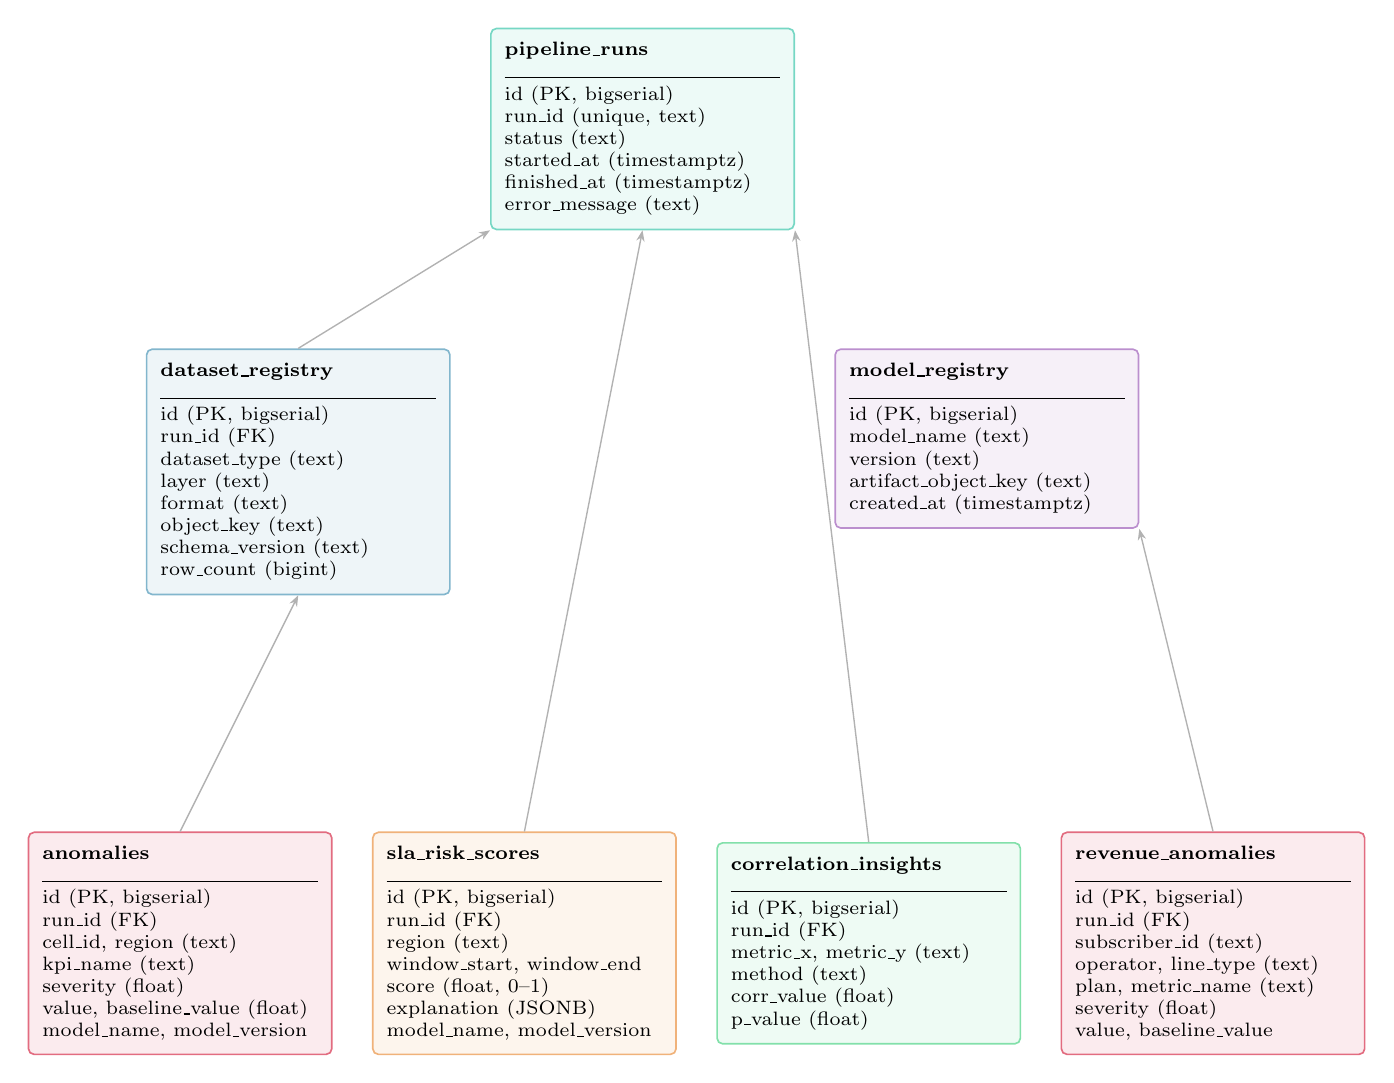
\begin{tikzpicture}[
  entity/.style={
    rectangle, rounded corners=2pt, draw=#1!60, fill=#1!8,
    minimum width=3.8cm, font=\scriptsize, align=left,
    inner sep=5pt, line width=0.6pt,
  },
  entity/.default={darkbg},
  entitytitle/.style={font=\scriptsize\bfseries, text=#1!80!black},
  entitytitle/.default={darkbg},
  fk/.style={-{Stealth[length=4pt]}, draw=gray!60, line width=0.5pt},
  node distance=1.2cm and 2cm,
]

  % Pipeline Runs (center top)
  \node[entity=cemteal] (runs) {
    \textbf{pipeline\_runs}\\
    \rule{3.5cm}{0.3pt}\\
    id (PK, bigserial)\\
    run\_id (unique, text)\\
    status (text)\\
    started\_at (timestamptz)\\
    finished\_at (timestamptz)\\
    error\_message (text)
  };
  
  % Dataset Registry
  \node[entity=ossblue, below left=1.5cm and 0.5cm of runs] (datasets) {
    \textbf{dataset\_registry}\\
    \rule{3.5cm}{0.3pt}\\
    id (PK, bigserial)\\
    run\_id (FK)\\
    dataset\_type (text)\\
    layer (text)\\
    format (text)\\
    object\_key (text)\\
    schema\_version (text)\\
    row\_count (bigint)
  };
  
  % Model Registry
  \node[entity=aiviolet, below right=1.5cm and 0.5cm of runs] (models) {
    \textbf{model\_registry}\\
    \rule{3.5cm}{0.3pt}\\
    id (PK, bigserial)\\
    model\_name (text)\\
    version (text)\\
    artifact\_object\_key (text)\\
    created\_at (timestamptz)
  };
  
  % Anomalies
  \node[entity=huaweired, below=3cm of datasets, xshift=-1.5cm] (anomalies) {
    \textbf{anomalies}\\
    \rule{3.5cm}{0.3pt}\\
    id (PK, bigserial)\\
    run\_id (FK)\\
    cell\_id, region (text)\\
    kpi\_name (text)\\
    severity (float)\\
    value, baseline\_value (float)\\
    model\_name, model\_version
  };
  
  % SLA Risk Scores
  \node[entity=cvmorange, right=0.5cm of anomalies] (sla) {
    \textbf{sla\_risk\_scores}\\
    \rule{3.5cm}{0.3pt}\\
    id (PK, bigserial)\\
    run\_id (FK)\\
    region (text)\\
    window\_start, window\_end\\
    score (float, 0--1)\\
    explanation (JSONB)\\
    model\_name, model\_version
  };
  
  % Correlation Insights
  \node[entity=bssgreen, right=0.5cm of sla] (corr) {
    \textbf{correlation\_insights}\\
    \rule{3.5cm}{0.3pt}\\
    id (PK, bigserial)\\
    run\_id (FK)\\
    metric\_x, metric\_y (text)\\
    method (text)\\
    corr\_value (float)\\
    p\_value (float)
  };
  
  % Revenue Anomalies
  \node[entity=huaweired, right=0.5cm of corr] (revanom) {
    \textbf{revenue\_anomalies}\\
    \rule{3.5cm}{0.3pt}\\
    id (PK, bigserial)\\
    run\_id (FK)\\
    subscriber\_id (text)\\
    operator, line\_type (text)\\
    plan, metric\_name (text)\\
    severity (float)\\
    value, baseline\_value
  };
  
  % Foreign Key arrows
  \draw[fk] (datasets.north) -- (runs.south west);
  \draw[fk] (anomalies.north) -- (datasets.south);
  \draw[fk] (sla.north) -- (runs.south);
  \draw[fk] (corr.north) -- (runs.south east);
  \draw[fk] (revanom.north) -- (models.south east);
  
\end{tikzpicture}
\caption{Entity-Relationship diagram of the PostgreSQL serving store (8 tables).}
\label{fig:er-diagram}
\end{figure}

\section{API Architecture}

The API Gateway exposes seven RESTful endpoints:

\begin{table}[H]
\centering
\caption{REST API endpoints.}
\label{tab:api-endpoints}
\begin{tabularx}{\textwidth}{@{}llX@{}}
\toprule
\textbf{Method} & \textbf{Path} & \textbf{Description} \\
\midrule
GET & \texttt{/health}              & Service liveness check \\
GET & \texttt{/sla-risk}            & Latest SLA risk score from GBR model \\
GET & \texttt{/sla-risk/history}    & Last N SLA risk scores, newest first \\
GET & \texttt{/anomalies}           & Latest N OSS anomaly records with cell\_id, severity \\
GET & \texttt{/pipeline-runs}       & Last N pipeline execution records \\
GET & \texttt{/revenue-anomalies}   & Latest N BSS revenue anomalies \\
GET & \texttt{/correlation}         & Latest N OSS$\leftrightarrow$BSS correlations (Pearson/Spearman) \\
\bottomrule
\end{tabularx}
\end{table}

The AI Service exposes four internal endpoints (not externally accessible in production):

\begin{table}[H]
\centering
\caption{AI Service internal endpoints.}
\label{tab:ai-endpoints}
\begin{tabularx}{\textwidth}{@{}lllX@{}}
\toprule
\textbf{Method} & \textbf{Path} & \textbf{Model} & \textbf{Output} \\
\midrule
GET  & \texttt{/health}                & ---   & Model version, status \\
POST & \texttt{/infer/sla-risk}        & GBR & Risk score $\in [0, 1]$ + feature importances \\
POST & \texttt{/infer/anomaly}         & IF  & Per-record anomaly flag + normalised severity \\
POST & \texttt{/infer/revenue-anomaly} & IF  & Per-record revenue anomaly flag + severity \\
\bottomrule
\end{tabularx}
\end{table}

\section{Chapter Summary}

This chapter described the system architecture at four levels: CEM--CVM positioning, container decomposition, pipeline orchestration, and data lake structure. The platform comprises five Docker containers orchestrating a 5-phase pipeline that transforms raw telecom data into actionable intelligence and autonomous recommendations. The next chapter details the data strategy: how real data from Tunisie Telecom is ingested, anonymised, and processed.

% ============================================================================
%  Chapter 5 --- Data Strategy
% ============================================================================
\chapter{Data Strategy}
\label{ch:data}

\section{Introduction}

The credibility of any AI system rests on the quality and authenticity of the data it is trained on. This chapter presents the project's data strategy: the real data sources from Tunisie Telecom and Huawei, the ingestion pipeline, the anonymisation process, the schema mapping, and the dual-mode architecture that allows the platform to operate on both real and synthetic data.

\section{Data Sources}

The platform ingests data from two primary sources and maintains a synthetic fallback:

\begin{table}[H]
\centering
\caption{Data sources and their characteristics.}
\label{tab:data-sources}
\begin{tabularx}{\textwidth}{@{}llllX@{}}
\toprule
\textbf{Source} & \textbf{Domain} & \textbf{Format} & \textbf{Status} & \textbf{Content} \\
\midrule
Tunisie Telecom & BSS & CSV / Excel & Real (provided via Huawei) & Subscriber profiles, ARPU, DOU, churn, plan types, revenue, usage \\
Tunisie Telecom & OSS & CSV / JSON & Real (provided via Huawei) & Cell-level KPIs: throughput, latency, packet loss, active users, RSRP \\
Huawei SmartCare & CEM & CSV / JSON & Real (export) & KQI, CEI scores, demarcation results, experience alerts \\
Synthetic Gen. & OSS + BSS & In-memory & Fallback / demo & Generated by pipeline-worker when no real data is available \\
\bottomrule
\end{tabularx}
\end{table}

\subsection{Why Real Data Matters}

The shift from synthetic-only to real operator data fundamentally changes the project's value:

\begin{itemize}
  \item \textbf{Before (synthetic):} Models were trained on artificially generated data with injected patterns. The anomalies were designed, the correlations were scripted, and the evaluation was circular --- the model could only ``discover'' what was explicitly injected.
  
  \item \textbf{After (real):} Models are trained on genuine network behaviour from a live Tunisian operator. The anomaly patterns are organic (not injected), the correlations are discovered (not scripted), and the evaluation metrics (precision, recall, F1) measure real detection capability.
  
  \item \textbf{Defence-proof:} When the jury asks "how do you know your model works?", the answer is: "it was trained on anonymised production data from Tunisie Telecom and validated against known network events."
\end{itemize}

\section{OSS Data Schema}

The following schema defines the expected structure of real OSS data from Tunisie Telecom. The exact number of records will depend on the dataset provided.

\begin{table}[H]
\centering
\caption{Expected OSS data schema (real TT data).}
\label{tab:oss-schema}
\begin{tabularx}{\textwidth}{@{}llcX@{}}
\toprule
\textbf{Source Column} & \textbf{Internal Field} & \textbf{Type} & \textbf{Description} \\
\midrule
cell\_id / eNodeB\_id     & \texttt{cell\_id}           & string  & Cell tower identifier \\
throughput\_dl\_mbps       & \texttt{throughput\_mbps}    & float   & Downlink throughput (Mbps) \\
latency\_rtt\_ms           & \texttt{latency\_ms}         & float   & Round-trip latency (ms) \\
packet\_loss\_pct          & \texttt{packet\_loss\_pct}   & float   & Packet loss percentage \\
active\_ue\_count          & \texttt{active\_users}       & int     & Number of active UEs on cell \\
rsrp\_dbm                  & \texttt{signal\_rsrp\_dbm}   & float   & Reference Signal Received Power (dBm) \\
region / site\_name        & \texttt{region}              & string  & Gouvernorat or site name \\
timestamp                  & \texttt{ts}                  & datetime & Measurement timestamp \\
\bottomrule
\end{tabularx}
\end{table}

\section{BSS Data Schema}

The BSS schema captures subscriber-level business metrics. The inclusion of APPU and DOU as explicit fields was directed by the supervisor to align with Huawei's BSS analytics framework.

\begin{table}[H]
\centering
\caption{Expected BSS data schema (real TT data).}
\label{tab:bss-schema}
\begin{tabularx}{\textwidth}{@{}llcX@{}}
\toprule
\textbf{Source Column} & \textbf{Internal Field} & \textbf{Type} & \textbf{Description} \\
\midrule
subscriber\_id / MSISDN & \texttt{subscriber\_id}  & string  & Anonymised subscriber identifier \\
operator                 & \texttt{operator}         & string  & Operator name (TT, Ooredoo, Orange) \\
line\_type               & \texttt{line\_type}       & string  & \texttt{prepaid} or \texttt{postpaid} \\
plan / forfait code      & \texttt{plan}             & string  & Subscription plan identifier \\
revenue (TND)            & \texttt{revenue\_tnd}     & float   & Monthly revenue in Tunisian Dinars \\
data\_usage\_gb           & \texttt{data\_used\_gb}   & float   & Monthly data consumption (GB) \\
voice\_minutes            & \texttt{voice\_min}       & float   & Monthly voice usage (minutes) \\
sms\_count                & \texttt{sms\_count}       & int     & Monthly SMS count \\
churn\_indicator          & \texttt{churn\_risk}      & float   & Churn risk score $\in [0, 1]$ \\
\textbf{appu\_tnd}       & \texttt{appu\_tnd}        & float   & Average Purchase Per User (TND) \\
\textbf{dou\_gb}         & \texttt{dou\_gb}          & float   & Data of Use --- monthly consumption (GB) \\
region / gouvernorat     & \texttt{region}            & string  & Subscriber's region \\
serving\_cell             & \texttt{serving\_cell}    & string  & Current serving cell (for OSS join) \\
timestamp / period       & \texttt{ts}               & datetime & Observation period \\
\bottomrule
\end{tabularx}
\end{table}

\section{Data Ingestion Pipeline}

% ── Figure: Data Ingestion Flow ───────────────────────────────────────────────
\begin{figure}[H]
\centering
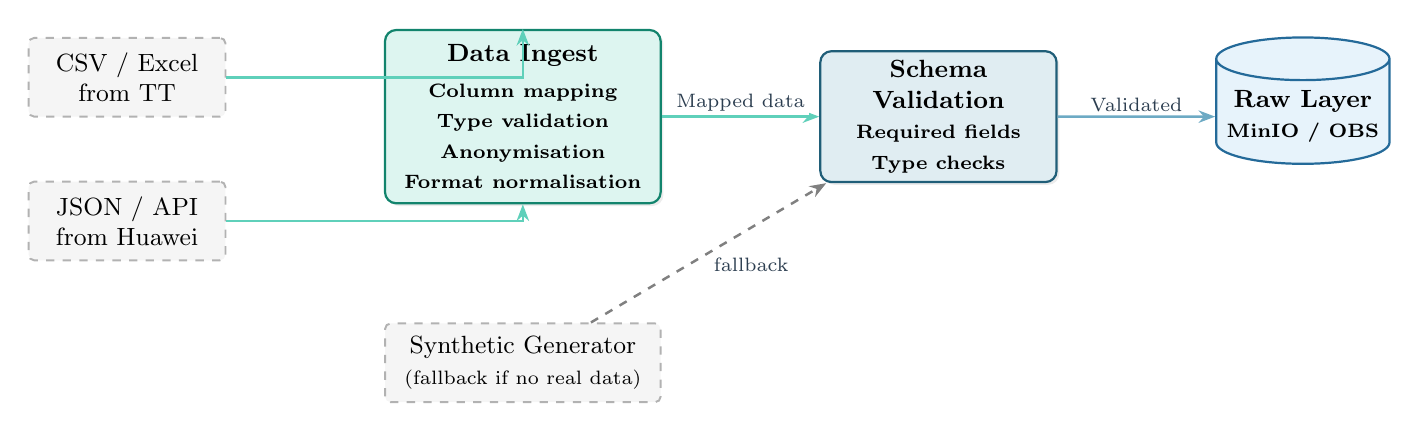
\begin{tikzpicture}[node distance=1.2cm and 2cm]

  % Source files
  \node[external, minimum width=2.5cm] (csv) {CSV / Excel\\from TT};
  \node[external, minimum width=2.5cm, below=0.8cm of csv] (json) {JSON / API\\from Huawei};
  
  % Ingestion service
  \node[service=cemteal, right=2cm of csv, yshift=-0.5cm, minimum width=3.5cm, minimum height=2.2cm] (ingest) {
    \textbf{Data Ingest}\\[2pt]
    {\scriptsize Column mapping}\\
    {\scriptsize Type validation}\\
    {\scriptsize Anonymisation}\\
    {\scriptsize Format normalisation}
  };
  
  % Schema validation
  \node[service=ossblue, right=2cm of ingest, minimum width=3cm] (validate) {
    \textbf{Schema}\\
    \textbf{Validation}\\
    {\scriptsize Required fields}\\
    {\scriptsize Type checks}
  };
  
  % Raw layer
  \node[datastore=datalake, right=2cm of validate] (rawlake) {
    \textbf{Raw Layer}\\{\scriptsize MinIO / OBS}
  };
  
  % Arrows
  \draw[myarrow=cemteal!70] (csv) -| (ingest);
  \draw[myarrow=cemteal!70] (json) -| (ingest);
  \draw[myarrow=cemteal!70] (ingest) -- (validate)
    node[arrlabel, midway, above] {Mapped data};
  \draw[myarrow=ossblue!70] (validate) -- (rawlake)
    node[arrlabel, midway, above] {Validated};
    
  % Synthetic fallback
  \node[external, below=1.5cm of ingest, minimum width=3.5cm] (synth) {
    Synthetic Generator\\{\scriptsize (fallback if no real data)}
  };
  \draw[myarrow=gray, dashed] (synth) -- (validate)
    node[arrlabel, midway, below right] {\scriptsize fallback};
    
\end{tikzpicture}
\caption{Data ingestion pipeline: real TT data is mapped, anonymised, validated, and stored in the raw lake layer. Synthetic generation is the fallback.}
\label{fig:data-ingestion}
\end{figure}

\subsection{Column Mapping}

The ingestion service performs column mapping from TT's native schema to the platform's internal schema. This mapping is configurable --- when TT provides data with different column names (e.g., \texttt{dl\_throughput} instead of \texttt{throughput\_dl\_mbps}), the mapping configuration is updated without code changes.

\subsection{Dual-Mode Operation}

The pipeline-worker operates in two modes, controlled by the environment variable \texttt{DATA\_SOURCE}:

\begin{itemize}
  \item \texttt{DATA\_SOURCE=real} (default): The worker reads real TT data files from a mounted volume (\texttt{/data/tt-import/}), applies anonymisation and column mapping, then proceeds with the standard 5-phase pipeline.
  \item \texttt{DATA\_SOURCE=synthetic}: The worker generates synthetic data using the built-in generators (retained from the earlier project phases). This mode is used for demos, testing, and when real data is not available.
\end{itemize}

\section{Anonymisation}

All personally identifiable information (PII) is removed or pseudonymised before the data enters the platform:

\begin{table}[H]
\centering
\caption{Anonymisation steps applied to incoming TT data.}
\label{tab:anonymisation}
\begin{tabularx}{\textwidth}{@{}llX@{}}
\toprule
\textbf{Field} & \textbf{Method} & \textbf{Rationale} \\
\midrule
MSISDN / subscriber\_id & SHA-256 hash with salt & Enables record linkage without exposing phone numbers \\
Name / address / NIN     & Strip entirely & Not required for analysis \\
Geographic precision     & Gouvernorat-level only & No GPS coordinates or precise addresses \\
Cell IDs                 & Optional opaque mapping & Map to anonymised IDs if TT requires \\
Temporal precision       & Minute-level preserved & Required for meaningful OSS--BSS correlation \\
\bottomrule
\end{tabularx}
\end{table}

The anonymisation is applied \emph{during ingestion}, before data reaches the raw layer. The raw layer thus contains already-anonymised data --- no PII exists anywhere in the platform.

\section{Feature Engineering}

Once raw data is ingested and stored, the pipeline performs feature engineering to transform it into ML-ready features.

\subsection{OSS Feature Engineering}

Each raw OSS record is enriched with computed fields:

\begin{itemize}
  \item \textbf{latency\_severity:} Categorical severity based on latency thresholds (\texttt{normal}, \texttt{warning}, \texttt{critical}).
  \item \textbf{throughput\_category:} Categorical label based on throughput ranges (\texttt{poor}, \texttt{fair}, \texttt{good}, \texttt{excellent}).
  \item \textbf{load\_factor:} $\text{active\_users} / \text{cell\_capacity}$ --- normalised cell utilisation.
  \item \textbf{qos\_score:} Composite quality score combining latency, throughput, and packet loss into a single $[0, 1]$ indicator.
\end{itemize}

For the SLA risk model, records are aggregated into \textbf{time windows} (per region, per time period) to produce 9 aggregate KPI features:

\begin{enumerate}
  \item \texttt{mean\_throughput\_mbps}
  \item \texttt{std\_throughput\_mbps}
  \item \texttt{mean\_latency\_ms}
  \item \texttt{std\_latency\_ms}
  \item \texttt{max\_latency\_ms}
  \item \texttt{mean\_packet\_loss\_pct}
  \item \texttt{max\_packet\_loss\_pct}
  \item \texttt{mean\_active\_users}
  \item \texttt{mean\_signal\_rsrp\_dbm}
\end{enumerate}

\subsection{BSS Feature Engineering}

Each BSS record is enriched with:

\begin{itemize}
  \item \textbf{arpu\_category:} \texttt{low} ($<$ 10 TND), \texttt{mid} ($<$ 40 TND), \texttt{high} ($\geq$ 40 TND)
  \item \textbf{data\_intensity:} Consumption brackets based on \texttt{dou\_gb}
  \item \textbf{churn\_bucket:} \texttt{safe}, \texttt{watch}, \texttt{risk}, \texttt{critical} based on \texttt{churn\_risk}
\end{itemize}

The BSS feature space for the revenue anomaly model includes 7 features:
\begin{enumerate}
  \item \texttt{revenue\_tnd}
  \item \texttt{data\_used\_gb}
  \item \texttt{voice\_min}
  \item \texttt{sms\_count}
  \item \texttt{churn\_risk}
  \item \texttt{appu\_tnd} (new --- Average Purchase Per User)
  \item \texttt{dou\_gb} (new --- Data of Use)
\end{enumerate}

\section{Data Quality and Validation}

Before processing, the ingestion service applies validation rules:

\begin{itemize}
  \item \textbf{Required fields:} All mandatory columns must be present (nulls are acceptable for optional fields).
  \item \textbf{Type checks:} Numeric fields must parse as floats/ints; timestamps must parse as ISO 8601 or common date formats.
  \item \textbf{Range checks:} Throughput $> 0$, latency $> 0$, packet loss $\in [0, 100]$, RSRP $\in [-140, -40]$ dBm.
  \item \textbf{Deduplication:} Exact duplicate records (same cell\_id + timestamp + all metrics) are removed.
\end{itemize}

Records that fail validation are logged but not silently dropped --- the pipeline reports the number of rejected records per run.

\section{Data Lineage and Traceability}

Every dataset produced by the pipeline is registered in the \texttt{dataset\_registry} table with:
\begin{itemize}
  \item The \texttt{run\_id} that produced it
  \item The \texttt{layer} (raw, processed, curated)
  \item The \texttt{object\_key} pointing to the MinIO/OBS object
  \item The \texttt{row\_count}
  \item The \texttt{schema\_version}
\end{itemize}

This enables full traceability: any anomaly or SLA risk score can be traced back to the exact raw data and pipeline run that produced it.

\section{Chapter Summary}

This chapter detailed the data strategy: real data from Tunisie Telecom and Huawei flows through an ingestion pipeline that anonymises, maps, validates, and stores data in a three-layer lake. The platform operates in dual mode (real or synthetic), ensuring robustness across deployment scenarios. The next chapter describes the AI models trained on this data.

% ============================================================================
%  Chapter 6 --- AI Models
% ============================================================================
\chapter{AI Models and Intelligence Layer}
\label{ch:ai}

\section{Introduction}

The intelligence layer of the AI Operations Agent comprises three machine learning models and one statistical correlation engine. Each addresses a distinct analytical need within the CEM--CVM bridge:

\begin{enumerate}
  \item \textbf{SLA Risk Prediction} --- supervised regression on aggregated OSS features.
  \item \textbf{Network (OSS) Anomaly Detection} --- unsupervised outlier detection on per-record KPIs.
  \item \textbf{Revenue (BSS) Anomaly Detection} --- unsupervised outlier detection on subscriber metrics.
  \item \textbf{OSS--BSS Correlation Engine} --- statistical analysis of metric pairs across domains.
\end{enumerate}

This chapter documents each model's design rationale, feature space, training methodology, and evaluation strategy.

\section{Model Overview}

% ── Figure: ML Model Pipeline ─────────────────────────────────────────────────
\begin{figure}[H]
\centering
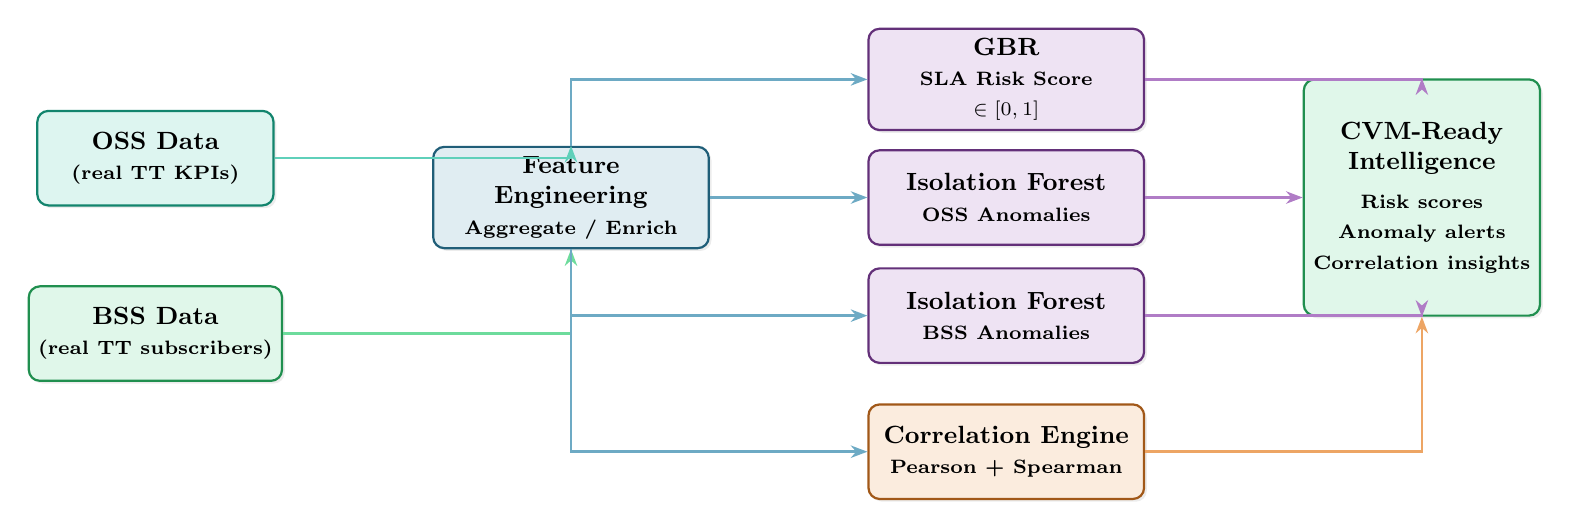
\begin{tikzpicture}[node distance=1.5cm and 1.8cm]

  % Input data
  \node[service=cemteal, minimum width=3cm] (ossdata) {OSS Data\\{\scriptsize (real TT KPIs)}};
  \node[service=bssgreen, minimum width=3cm, below=1cm of ossdata] (bssdata) {BSS Data\\{\scriptsize (real TT subscribers)}};
  
  % Feature engineering
  \node[service=ossblue, right=2cm of ossdata, minimum width=3.5cm, yshift=-0.5cm] (feat) {
    \textbf{Feature}\\
    \textbf{Engineering}\\
    {\scriptsize Aggregate / Enrich}
  };
  
  % Models
  \node[service=aiviolet, right=2cm of feat, yshift=1.5cm, minimum width=3.5cm] (gbr) {
    \textbf{GBR}\\
    {\scriptsize SLA Risk Score}\\
    {\scriptsize $\in [0, 1]$}
  };
  \node[service=aiviolet, right=2cm of feat, yshift=0cm, minimum width=3.5cm] (ifoss) {
    \textbf{Isolation Forest}\\
    {\scriptsize OSS Anomalies}
  };
  \node[service=aiviolet, right=2cm of feat, yshift=-1.5cm, minimum width=3.5cm] (ifbss) {
    \textbf{Isolation Forest}\\
    {\scriptsize BSS Anomalies}
  };
  
  % Correlation
  \node[service=cvmorange, below=0.5cm of ifbss, minimum width=3.5cm] (corr) {
    \textbf{Correlation Engine}\\
    {\scriptsize Pearson + Spearman}
  };
  
  % Outputs
  \node[service=bssgreen, right=2cm of ifoss, minimum width=3cm, minimum height=3cm] (output) {
    \textbf{CVM-Ready}\\
    \textbf{Intelligence}\\[3pt]
    {\scriptsize Risk scores}\\
    {\scriptsize Anomaly alerts}\\
    {\scriptsize Correlation insights}
  };
  
  % Arrows
  \draw[myarrow=cemteal!70] (ossdata) -| (feat);
  \draw[myarrow=bssgreen!70] (bssdata) -| (feat);
  \draw[myarrow=ossblue!70] (feat) |- (gbr);
  \draw[myarrow=ossblue!70] (feat) -- (ifoss);
  \draw[myarrow=ossblue!70] (feat) |- (ifbss);
  \draw[myarrow=ossblue!70] (feat) |- (corr);
  \draw[myarrow=aiviolet!70] (gbr) -| (output);
  \draw[myarrow=aiviolet!70] (ifoss) -- (output);
  \draw[myarrow=aiviolet!70] (ifbss) -| (output);
  \draw[myarrow=cvmorange!70] (corr) -| (output);
  
\end{tikzpicture}
\caption{ML model pipeline: from raw data through feature engineering to CVM-ready intelligence.}
\label{fig:ml-pipeline}
\end{figure}

\begin{table}[H]
\centering
\caption{Model inventory: three ML models and one statistical engine.}
\label{tab:model-overview}
\begin{tabularx}{\textwidth}{@{}llllX@{}}
\toprule
\textbf{Model} & \textbf{Algorithm} & \textbf{Type} & \textbf{Features} & \textbf{Output} \\
\midrule
SLA Risk Scorer & GradientBoostingRegressor & Supervised regression & 9 aggregate OSS & Risk score $\in [0, 1]$ + importances \\
OSS Anomaly & IsolationForest & Unsupervised & 5 per-record OSS & Anomaly flag + severity $\in [0, 1]$ \\
BSS Anomaly & IsolationForest & Unsupervised & 7 per-record BSS & Anomaly flag + severity $\in [0, 1]$ \\
Correlation & Pearson + Spearman & Statistical & 5 OSS--BSS pairs & 10 correlation coefficients + p-values \\
\bottomrule
\end{tabularx}
\end{table}

\section{Model 1: SLA Risk Prediction (GradientBoostingRegressor)}

\subsection{Business Objective}

Predict the risk that a current KPI time window will lead to an SLA (Service Level Agreement) breach. The output is a continuous score in $[0.0, 1.0]$, where 0 indicates nominal performance and 1 indicates imminent SLA violation. This score maps directly to SmartCare's experience risk concept and feeds CVM retention decision-making.

\subsection{Why Gradient Boosting}

Table~\ref{tab:gbr-justification} justifies the model choice:

\begin{table}[H]
\centering
\caption{Justification for GradientBoostingRegressor.}
\label{tab:gbr-justification}
\begin{tabularx}{\textwidth}{@{}lX@{}}
\toprule
\textbf{Criterion} & \textbf{Rationale} \\
\midrule
Data type & Tabular, numeric --- GBR's strongest domain \\
Non-linearity & SLA risk has threshold-driven, non-linear dynamics (e.g., latency only matters after a threshold) \\
Feature interactions & High latency + packet loss is worse than either alone --- GBR captures this \\
Dataset size & Small-to-medium --- GBR excels; neural networks would overfit \\
Explainability & \texttt{feature\_importances\_} enables direct explanation during defence \\
Maturity & Well-understood, battle-tested, academically defensive \\
\bottomrule
\end{tabularx}
\end{table}

\subsection{Input Features (9 Aggregate OSS KPIs)}

The model takes as input an aggregated KPI feature vector per time window per region:

$$\mathbf{x} = \begin{bmatrix} \bar{T} & \sigma_T & \bar{L} & \sigma_L & L_{\max} & \bar{P} & P_{\max} & \bar{U} & \bar{S} \end{bmatrix}$$

Where $T$ = throughput (Mbps), $L$ = latency (ms), $P$ = packet loss (\%), $U$ = active users, $S$ = RSRP (dBm). Bars denote means, $\sigma$ denotes standard deviations.

\subsection{Target Variable}

The risk label $y \in [0, 1]$ is constructed from the features using a domain-knowledge-driven formula:

\begin{align}
y &= \text{clip}\!\left(\frac{\bar{L} - 20}{60},\; 0,\; 0.35\right) 
   + \text{clip}\!\left(\frac{L_{\max} - 30}{70},\; 0,\; 0.25\right) \nonumber\\
  &+ \text{clip}\!\left(\frac{\bar{P}}{4},\; 0,\; 0.25\right)
   + \text{clip}\!\left(\frac{P_{\max}}{6},\; 0,\; 0.15\right) \nonumber\\
  &+ \text{clip}\!\left(\frac{60 - \bar{T}}{100},\; 0,\; 0.20\right)
   + \epsilon, \quad \epsilon \sim \mathcal{N}(0, 0.03)
\label{eq:risk-label}
\end{align}

This formula encodes telecom domain knowledge: latency contributes risk only above a threshold (20~ms for mean, 30~ms for max), packet loss always contributes proportionally, low throughput (below 60~Mbps) adds risk, and a small noise term $\epsilon$ prevents the model from learning a trivially deterministic function.

With real TT data, this label construction is applied to the actual observed KPI values --- the model learns from \emph{real} degradation patterns, not synthetic injections.

\subsection{Training Pipeline}

\begin{lstlisting}[language=Python, caption={SLA Risk model training pipeline.}]
Pipeline([
    ("scaler", StandardScaler()),
    ("gbr", GradientBoostingRegressor(
        n_estimators=200,
        max_depth=4,
        learning_rate=0.05,
        subsample=0.8,
        random_state=42,
    )),
])
\end{lstlisting}

\subsection{Hyperparameters}

\begin{table}[H]
\centering
\caption{GBR hyperparameters and their roles.}
\label{tab:gbr-hyperparams}
\begin{tabularx}{\textwidth}{@{}llcX@{}}
\toprule
\textbf{Hyperparameter} & \textbf{Value} & \textbf{Tunable} & \textbf{Effect} \\
\midrule
\texttt{n\_estimators}  & 200  & Yes & Number of boosting stages \\
\texttt{max\_depth}     & 4    & Yes & Depth of each weak tree (complexity control) \\
\texttt{learning\_rate} & 0.05 & Yes & Contribution of each tree (lower = more stable) \\
\texttt{subsample}      & 0.8  & Yes & Stochastic sampling per stage (regularisation) \\
\texttt{random\_state}  & 42   & No  & Reproducibility seed \\
\bottomrule
\end{tabularx}
\end{table}

\subsection{Feature Importances and Explainability}

GBR provides \texttt{feature\_importances\_} --- the normalised total reduction of the loss function contributed by each feature. In practice, \texttt{mean\_latency\_ms} dominates (importance $\sim 0.69$), consistent with the risk label construction and real telecom behaviour: latency is the primary driver of subscriber experience degradation.

The feature importances are returned as part of every SLA risk inference response, enabling CVM systems (or human analysts) to understand \emph{why} the risk score is high or low.

\subsection{Evaluation Metrics}

For the SLA risk model (supervised regression):
\begin{itemize}
  \item \textbf{MAE} (Mean Absolute Error): Average magnitude of prediction errors, in risk-score units.
  \item \textbf{RMSE} (Root Mean Squared Error): Penalises larger errors more heavily.
  \item \textbf{$R^2$} (Coefficient of Determination): Proportion of variance explained by the model.
\end{itemize}

With real data, we use a train/validation/test split to obtain unbiased estimates.

\section{Model 2: OSS Anomaly Detection (IsolationForest)}

\subsection{Business Objective}

Detect abnormal network KPI records --- throughput collapses, latency spikes, packet loss surges, cell overloads, or weak signal conditions --- \emph{without} requiring labelled data. This corresponds to SmartCare's demarcation function: identifying \emph{which cells} are experiencing abnormal behaviour.

\subsection{Why Isolation Forest}

\begin{itemize}
  \item \textbf{No labels required:} In real telecom operations, comprehensive anomaly labels are rarely available. IsolationForest learns the ``normal'' distribution and flags deviations.
  \item \textbf{Speed and scalability:} Linear time complexity $O(n \cdot t \cdot \psi)$ where $t$ = trees, $\psi$ = subsample size.
  \item \textbf{Dual output:} Provides both a binary decision (normal/anomaly) and a continuous anomaly score for severity ranking.
  \item \textbf{Interpretable:} Anomaly score = normalised inverse of average path length. Shorter paths = more anomalous.
\end{itemize}

\subsection{Input Features (5 Per-Record OSS KPIs)}

$$\mathbf{x} = \begin{bmatrix} T & L & P & U & S \end{bmatrix}$$

Where $T$ = throughput, $L$ = latency, $P$ = packet loss, $U$ = active users, $S$ = RSRP. Each record represents one cell at one point in time.

\subsection{Anomaly Score Normalisation}

The raw IsolationForest \texttt{decision\_function} output is more negative for more anomalous records. We normalise to $[0, 1]$ where 1 = most anomalous:

$$\text{severity}_i = 1 - \frac{s_i - s_{\min}}{s_{\max} - s_{\min} + \epsilon}$$

where $s_i$ is the raw score and $\epsilon = 10^{-9}$ prevents division by zero.

\subsection{Contamination Parameter}

The \texttt{contamination} parameter defines the expected proportion of anomalies in the dataset. This is the \emph{most sensitive} hyperparameter in IsolationForest:

\begin{itemize}
  \item In real operator data, anomalies are typically rarer than the 5\% used in synthetic training. We anticipate contamination values in the range $[0.01, 0.03]$ for real TT data.
  \item The exact value will be calibrated during the retraining phase, using validation against known network events or operator-labelled incidents.
\end{itemize}

\subsection{Training Pipeline}

\begin{lstlisting}[language=Python, caption={OSS Anomaly model training pipeline.}]
Pipeline([
    ("scaler", StandardScaler()),
    ("ifo", IsolationForest(
        n_estimators=150,
        contamination=0.05,  # adjusted for real data
        random_state=42,
    )),
])
\end{lstlisting}

\subsection{Handling Class Imbalance in Real Data}

Real anomalies in production telecom networks are significantly rarer than the 5\% synthetic injection rate. Strategies for handling this:

\begin{enumerate}
  \item \textbf{Lower contamination:} Reduce to $0.01$--$0.03$ to match real prevalence.
  \item \textbf{Sliding threshold:} Instead of using the built-in decision threshold, apply a percentile-based threshold on anomaly scores.
  \item \textbf{Operator-guided calibration:} If TT provides a list of known incident dates/cells, we calibrate the threshold to maximise detection of those known events.
\end{enumerate}

\section{Model 3: BSS Revenue Anomaly Detection (IsolationForest)}

\subsection{Business Objective}

Detect anomalous subscriber-level business behaviour:
\begin{itemize}
  \item Abnormal recharge patterns (very high = potential SIM box fraud; very low = dormant SIM)
  \item Excessive data consumption outside normal plan bounds
  \item SMS spam patterns (very high SMS count)
  \item SIM-box-like voice patterns (very high voice minutes)
  \item Abrupt churn-risk spikes correlated with network events
\end{itemize}

This model is the BSS-side complement to the OSS anomaly detector. Together, they provide the AI Agent with a 360° view of both network and business anomalies.

\subsection{Input Features (7 Per-Record BSS Metrics)}

$$\mathbf{x} = \begin{bmatrix} R & D & V & S & C & A & G \end{bmatrix}$$

Where $R$ = revenue\_tnd, $D$ = data\_used\_gb, $V$ = voice\_min, $S$ = sms\_count, $C$ = churn\_risk, $A$ = appu\_tnd, $G$ = dou\_gb.

The inclusion of APPU and DOU (supervisor-directed) expands the feature space from 5 to 7, providing richer subscriber characterisation for anomaly detection.

\subsection{Training Pipeline}

\begin{lstlisting}[language=Python, caption={BSS Revenue Anomaly model training pipeline.}]
Pipeline([
    ("scaler", StandardScaler()),
    ("ifo", IsolationForest(
        n_estimators=150,
        contamination=0.05,  # adjusted for real data
        random_state=42,
    )),
])
\end{lstlisting}

\section{Model 4: OSS--BSS Correlation Engine}

\subsection{Objective}

Quantify the statistical relationship between network degradation and business impact. This is the \textbf{O+B convergence demonstration}: showing, with statistical evidence, that when the network degrades, revenue suffers.

\subsection{Metric Pairs}

The engine computes correlations on five OSS--BSS metric pairs:

\begin{table}[H]
\centering
\caption{OSS--BSS correlation pairs.}
\label{tab:corr-pairs}
\begin{tabular}{@{}lll@{}}
\toprule
\textbf{OSS Metric ($x$)} & \textbf{BSS Metric ($y$)} & \textbf{Expected Direction} \\
\midrule
\texttt{throughput\_mbps}    & \texttt{revenue\_tnd}   & Positive (higher throughput $\to$ higher revenue) \\
\texttt{latency\_ms}         & \texttt{revenue\_tnd}   & Negative (higher latency $\to$ lower revenue) \\
\texttt{packet\_loss\_pct}   & \texttt{churn\_risk}    & Positive (more loss $\to$ higher churn) \\
\texttt{latency\_ms}         & \texttt{data\_used\_gb} & Negative (higher latency $\to$ less data use) \\
\texttt{signal\_rsrp\_dbm}   & \texttt{revenue\_tnd}   & Positive (better signal $\to$ higher revenue) \\
\bottomrule
\end{tabular}
\end{table}

\subsection{Statistical Methods}

For each pair, we compute:

\begin{itemize}
  \item \textbf{Pearson $r$:} Measures linear correlation:
  $$r = \frac{\sum_{i=1}^{n}(x_i - \bar{x})(y_i - \bar{y})}{\sqrt{\sum(x_i - \bar{x})^2 \cdot \sum(y_i - \bar{y})^2}}$$
  
  \item \textbf{Spearman $\rho$:} Measures monotonic (rank-based) correlation --- captures non-linear but consistent trends.
\end{itemize}

Both methods return a correlation coefficient ($\in [-1, 1]$) and a p-value indicating statistical significance. With real TT data, these coefficients reflect \emph{actual} network-to-business relationships in the Tunisian market --- a finding of publishable quality.

\subsection{Output}

Each pipeline run produces \textbf{10 correlation results} (5 pairs $\times$ 2 methods), persisted to the \texttt{correlation\_insights} table with full traceability (run\_id, time window, p-values).

\section{Model Training on Real Data}

\subsection{Retraining Strategy}

The transition from synthetic to real data follows a phased approach:

\begin{enumerate}
  \item \textbf{Phase 1 (current):} Models are trained with v2.0 on synthetic data at $N = 3000$ samples. This establishes the architecture and inference pipeline.
  \item \textbf{Phase 2 (pending real data):} Models are retrained as v3.0 on real TT data. The number of training samples, time windows, and anomaly prevalence will be determined by the actual dataset size. Key adjustments:
  \begin{itemize}
    \item IsolationForest contamination reduced to $[0.01, 0.03]$
    \item GBR risk labels computed from real KPI observations
    \item BSS model expanded to 7 features (adding APPU, DOU)
  \end{itemize}
\end{enumerate}

\subsection{Model Persistence and Versioning}

Trained models are serialised as \texttt{.joblib} files and stored on a Docker volume (\texttt{/app/models/}). The AI service loads existing models on startup; retraining occurs only when models are absent or when a version bump is triggered.

Model versions:
\begin{itemize}
  \item \textbf{v2.0:} Synthetic-trained (current, operational)
  \item \textbf{v3.0:} Real-data-trained (pending data delivery)
\end{itemize}

\section{Evaluation Framework}

\subsection{SLA Risk Model (Supervised)}

\begin{itemize}
  \item Train/validation/test split (e.g., 70/15/15 or time-based)
  \item Metrics: MAE, RMSE, $R^2$ on held-out test set
  \item Feature importance analysis for explainability
\end{itemize}

\subsection{Anomaly Models (Unsupervised)}

When labelled validation data is available (known incidents from TT):
\begin{itemize}
  \item \textbf{Precision:} Of all records flagged as anomalies, what fraction are true anomalies?
  \item \textbf{Recall:} Of all true anomalies, what fraction were detected?
  \item \textbf{F1 Score:} Harmonic mean of precision and recall.
  \item \textbf{Confusion matrix:} True positives, false positives, true negatives, false negatives.
\end{itemize}

When labels are unavailable:
\begin{itemize}
  \item Inject known synthetic anomalies into real data and measure detection rate.
  \item Monitor false positive rate on known-stable periods.
  \item Use anomaly score distribution analysis (bimodal distribution implies good separation).
\end{itemize}

\subsection{Correlation Engine}

\begin{itemize}
  \item Statistical significance: p-value $< 0.05$ for meaningful correlations.
  \item Comparison of Pearson vs. Spearman to identify non-linear relationships.
  \item Cross-temporal stability: correlations should be consistent across different time windows.
\end{itemize}

\section{Chapter Summary}

This chapter documented the four components of the intelligence layer: GBR for SLA risk prediction, two IsolationForest models for OSS and BSS anomaly detection, and a Pearson/Spearman correlation engine for O+B convergence. Each model's design, features, training pipeline, and evaluation framework were detailed. With real TT data, these models transition from academic demonstrations to industrial-grade analytics tools. The next chapter covers the implementation details.

% ============================================================================
%  Chapter 7 --- Implementation
% ============================================================================
\chapter{Implementation}
\label{ch:implementation}

\section{Introduction}

This chapter details the technical implementation of the AI Operations Agent platform: the technology stack, service implementations, Docker composition, database schema deployment, and the end-to-end execution walkthrough. Every component described here is operational and containerised.

\section{Technology Stack}

\begin{table}[H]
\centering
\caption{Technology stack.}
\label{tab:tech-stack}
\begin{tabularx}{\textwidth}{@{}llX@{}}
\toprule
\textbf{Component} & \textbf{Technology} & \textbf{Version / Notes} \\
\midrule
Language          & Python 3                & All services written in Python \\
Web framework     & FastAPI                 & API Gateway + AI Service \\
ML library        & scikit-learn            & 1.5.2 (pinned in requirements.txt) \\
Data processing   & NumPy, pandas           & Feature engineering + data transforms \\
Serialisation     & joblib                  & Model persistence \\
Database          & PostgreSQL              & 16 (official Docker image) \\
Object storage    & MinIO                   & S3-compatible (official Docker image) \\
Containerisation  & Docker + Docker Compose & Multi-service orchestration \\
HTTP client       & httpx (async-capable)   & Pipeline worker $\to$ AI service calls \\
DB client         & psycopg2                & PostgreSQL driver \\
S3 client         & boto3                   & MinIO/OBS interaction \\
\bottomrule
\end{tabularx}
\end{table}

\section{Project Structure}

The repository follows a monorepo structure with each service in its own directory:

\begin{lstlisting}[language=bash, caption={Repository structure.}, label={lst:repo-structure}]
telecom-cloud-intelligence/
  docker-compose.yml
  services/
    api-gateway/
      Dockerfile
      main.py               # FastAPI (7 endpoints)
      requirements.txt
    ai-service/
      Dockerfile
      main.py               # ML models + 4 endpoints
      requirements.txt
    pipeline-worker/
      Dockerfile
      requirements.txt
      worker/
        __main__.py          # 5-phase pipeline
  docs/
    db/schema.sql            # PostgreSQL DDL
    architecture/            # Architecture docs
    data-model/              # Data lake + ER docs
  report/                    # This LaTeX report
  infra/                     # Infrastructure configs
\end{lstlisting}

\section{Service Implementation Details}

\subsection{API Gateway (\texttt{services/api-gateway/main.py})}

The API Gateway is a stateless, read-only service. It connects to PostgreSQL and serves the latest results for each analytical endpoint. Key implementation decisions:

\begin{itemize}
  \item \textbf{No cache layer:} Results are read directly from PostgreSQL. The data volume is small enough that query latency is negligible.
  \item \textbf{Pagination:} All list endpoints accept a \texttt{limit} parameter with sensible bounds (\texttt{ge=1, le=200/500}).
  \item \textbf{Error handling:} HTTP exceptions are propagated cleanly; internal errors return 500 with a message.
\end{itemize}

\begin{lstlisting}[language=Python, caption={API Gateway --- SLA risk endpoint (excerpt).}]
@app.get("/sla-risk")
def sla_risk_latest():
    with get_conn() as conn:
        with conn.cursor(cursor_factory=RealDictCursor) as cur:
            cur.execute("""
                SELECT id, run_id, region, window_start, window_end,
                       score, explanation, model_name, model_version,
                       created_at
                FROM sla_risk_scores
                ORDER BY created_at DESC LIMIT 1;
            """)
            row = cur.fetchone()
            if not row:
                raise HTTPException(404, "No SLA risk scores")
            return row
\end{lstlisting}

\subsection{AI Service (\texttt{services/ai-service/main.py})}

The AI Service hosts the three ML models and exposes inference endpoints. Key implementation decisions:

\begin{itemize}
  \item \textbf{Train-once, serve-many:} Models are trained on first startup (if no persisted artifacts exist) and reloaded on subsequent restarts from \texttt{/app/models/*.joblib}.
  \item \textbf{Docker volume (\texttt{aimodels}):} Model artifacts survive container restarts.
  \item \textbf{Deterministic fallback:} If the pipeline worker calls \texttt{/infer/sla-risk} without features, a deterministic hash-based score is returned (clearly marked as non-model-based).
  \item \textbf{Anomaly score normalisation:} Raw IsolationForest \texttt{decision\_function} scores are normalised to $[0, 1]$ for severity representation.
\end{itemize}

\begin{lstlisting}[language=Python, caption={AI Service --- IsolationForest inference (excerpt).}]
@app.post("/infer/anomaly")
def infer_anomaly(req: AnomalyRequest):
    X = np.array([
        [r.throughput_mbps, r.latency_ms, r.packet_loss_pct,
         float(r.active_users), r.signal_rsrp_dbm]
        for r in req.records
    ])
    labels = _anomaly_model.predict(X)  # +1 or -1
    raw_scores = _anomaly_model.decision_function(X)
    score_range = raw_scores.max() - raw_scores.min()
    norm_scores = 1.0 - (raw_scores - raw_scores.min()) \
                        / (score_range + 1e-9)
    # ... return anomaly results ...
\end{lstlisting}

\subsection{Pipeline Worker (\texttt{services/pipeline-worker/worker/\_\_main\_\_.py})}

The pipeline worker is a run-once container that executes the full 5-phase data pipeline. It orchestrates all other services:

\begin{enumerate}
  \item Creates MinIO buckets if they do not exist.
  \item Ingests data (real from \texttt{/data/tt-import/} or synthetic as fallback).
  \item Uploads raw data to MinIO \texttt{raw} bucket.
  \item Registers the pipeline run and datasets in PostgreSQL.
  \item Performs feature engineering (OSS: severity, QoS; BSS: ARPU category, intensity).
  \item Calls the AI Service for SLA risk inference.
  \item Calls the AI Service for OSS anomaly detection.
  \item Calls the AI Service for BSS revenue anomaly detection.
  \item Computes OSS--BSS statistical correlations.
  \item Builds the curated dataset and uploads to MinIO \texttt{curated} bucket.
  \item Persists all results to PostgreSQL.
  \item Registers model versions and marks the pipeline as succeeded.
\end{enumerate}

\section{Docker Compose Orchestration}

\begin{lstlisting}[language=yaml, caption={Docker Compose configuration (simplified).}]
services:
  postgres:
    image: postgres:16
    environment:
      POSTGRES_DB: telecom_intel
      POSTGRES_USER: telecom
      POSTGRES_PASSWORD: telecom_pw
    healthcheck:
      test: ["CMD-SHELL", "pg_isready -U telecom"]
    volumes:
      - pgdata:/var/lib/postgresql/data

  minio:
    image: minio/minio:latest
    command: server /data --console-address ":9001"
    healthcheck:
      test: ["CMD", "curl", "-f", 
             "http://localhost:9000/minio/health/live"]
    volumes:
      - miniodata:/data

  api-gateway:
    build: ./services/api-gateway
    ports: ["8000:8000"]
    depends_on:
      postgres: { condition: service_healthy }

  ai-service:
    build: ./services/ai-service
    ports: ["8001:8001"]
    volumes:
      - aimodels:/app/models
    depends_on:
      postgres: { condition: service_healthy }

  pipeline-worker:
    build: ./services/pipeline-worker
    depends_on:
      postgres: { condition: service_healthy }
      minio:    { condition: service_healthy }

volumes:
  pgdata:
  miniodata:
  aimodels:
\end{lstlisting}

\subsection{Health Checks and Dependencies}

Docker Compose health checks ensure services start in the correct order:
\begin{itemize}
  \item PostgreSQL must be healthy (\texttt{pg\_isready}) before API Gateway, AI Service, and Pipeline Worker start.
  \item MinIO must be healthy (HTTP liveness endpoint) before Pipeline Worker starts.
  \item The pipeline worker depends on both infrastructure services and the AI service (for inference calls).
\end{itemize}

\subsection{Named Volumes}

Three named volumes ensure data persistence across container restarts:
\begin{itemize}
  \item \texttt{pgdata} --- PostgreSQL data directory
  \item \texttt{miniodata} --- MinIO object storage
  \item \texttt{aimodels} --- Trained ML model artifacts (\texttt{.joblib} files)
\end{itemize}

\section{Database Schema Deployment}

The PostgreSQL schema is applied on first connection by the pipeline worker or via the \texttt{schema.sql} DDL file. Eight tables are created:

\begin{lstlisting}[language=SQL, caption={Key schema definitions (excerpt).}]
CREATE TABLE IF NOT EXISTS pipeline_runs (
  id         BIGSERIAL PRIMARY KEY,
  run_id     TEXT NOT NULL UNIQUE,
  status     TEXT NOT NULL DEFAULT 'started',
  started_at TIMESTAMPTZ NOT NULL DEFAULT now(),
  finished_at TIMESTAMPTZ,
  error_message TEXT
);

CREATE TABLE IF NOT EXISTS sla_risk_scores (
  id            BIGSERIAL PRIMARY KEY,
  run_id        TEXT REFERENCES pipeline_runs(run_id),
  region        TEXT,
  window_start  TIMESTAMPTZ,
  window_end    TIMESTAMPTZ,
  score         DOUBLE PRECISION CHECK (score >= 0 AND score <= 1),
  explanation   JSONB,
  model_name    TEXT DEFAULT 'sla-risk',
  model_version TEXT,
  created_at    TIMESTAMPTZ DEFAULT now()
);
\end{lstlisting}

\section{End-to-End Execution Walkthrough}

A complete platform execution follows these steps:

\begin{enumerate}
  \item \textbf{Start:} \texttt{docker compose up --build}
  \item PostgreSQL and MinIO start and become healthy.
  \item AI Service starts, loads/trains models, serves on port 8001.
  \item API Gateway starts, connects to PostgreSQL, serves on port 8000.
  \item Pipeline Worker starts:
  \begin{itemize}
    \item Checks for real TT data in \texttt{/data/tt-import/}
    \item If present: ingests, anonymises, maps to schema
    \item If absent: generates synthetic data (fallback)
    \item Executes 5-phase pipeline
  \end{itemize}
  \item \textbf{Query results:}
  \begin{itemize}
    \item \texttt{curl http://localhost:8000/sla-risk} --- latest SLA risk score
    \item \texttt{curl http://localhost:8000/anomalies} --- detected anomalies
    \item \texttt{curl http://localhost:8000/revenue-anomalies} --- BSS anomalies
    \item \texttt{curl http://localhost:8000/correlation} --- OSS--BSS correlations
  \end{itemize}
\end{enumerate}

\section{Chapter Summary}

This chapter detailed the technical implementation: Python/FastAPI services, scikit-learn models, Docker Compose orchestration, PostgreSQL schema, and the end-to-end execution flow. All services are fully containerised, use health checks for dependency management, and persist data across restarts through named volumes. The next chapter presents the evaluation results.

% ============================================================================
%  Chapter 8 --- Evaluation and Results
% ============================================================================
\chapter{Evaluation and Results}
\label{ch:evaluation}

\section{Introduction}

This chapter presents the evaluation framework and results for the AI Operations Agent platform. We evaluate the system at three levels: model performance metrics (Section~\ref{sec:eval-models}), correlation analysis findings (Section~\ref{sec:eval-correlation}), and end-to-end platform validation (Section~\ref{sec:eval-e2e}).

The specific numerical results (precision, recall, F1, correlation coefficients, confusion matrices) will be populated once the real Tunisie Telecom data is fully ingested and the v3.0 models are trained. The evaluation \emph{framework} and methodology are established here.

\section{Model Evaluation}
\label{sec:eval-models}

\subsection{SLA Risk Model Evaluation}

\subsubsection{Methodology}

The GradientBoostingRegressor is evaluated using a held-out test split:

\begin{itemize}
  \item \textbf{Split strategy:} Time-based split recommended (train on older windows, test on recent windows) to simulate realistic deployment. Alternative: random 70/15/15 split.
  \item \textbf{Metrics:} MAE, RMSE, $R^2$.
  \item \textbf{Baseline comparison:} Compare against a naive baseline (e.g., mean risk score) to demonstrate model value.
\end{itemize}

\subsubsection{Results Framework}

\begin{table}[H]
\centering
\caption{SLA Risk Model evaluation results.}
\label{tab:sla-results}
\begin{tabular}{@{}lcc@{}}
\toprule
\textbf{Metric} & \textbf{v2.0 (Synthetic)} & \textbf{v3.0 (Real TT Data)} \\
\midrule
MAE   & \textit{measured} & \textit{pending real data} \\
RMSE  & \textit{measured} & \textit{pending real data} \\
$R^2$ & \textit{measured} & \textit{pending real data} \\
\bottomrule
\end{tabular}
\end{table}

\subsubsection{Feature Importance Analysis}

% ── Figure: Feature Importance Bar Chart (TikZ/pgfplots) ─────────────────────
\begin{figure}[H]
\centering
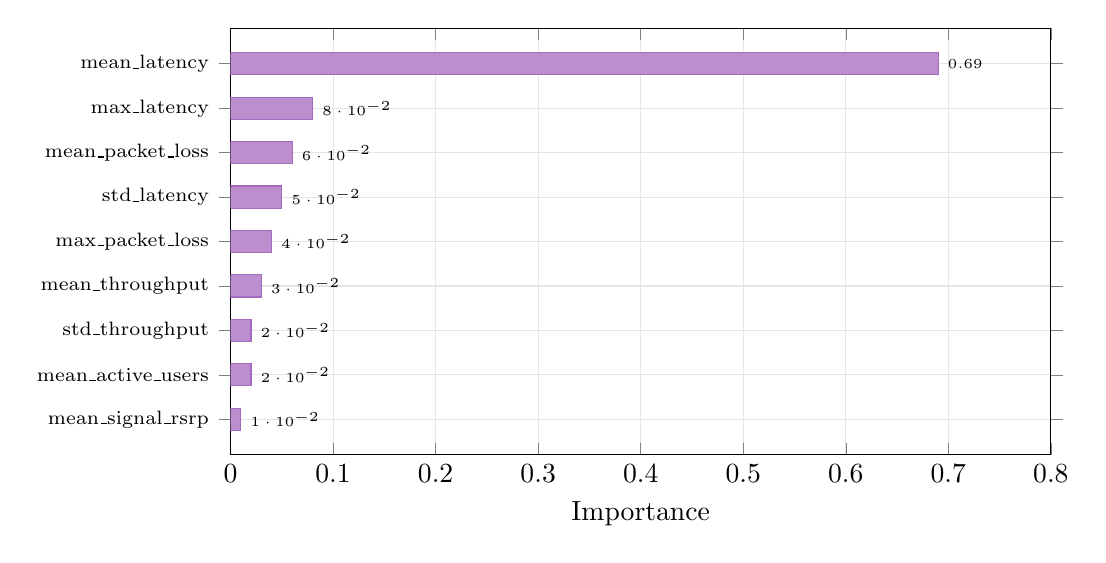
\begin{tikzpicture}
\begin{axis}[
    xbar,
    width=12cm,
    height=7cm,
    xlabel={Importance},
    ylabel={},
    symbolic y coords={
      {mean\_signal\_rsrp},
      {mean\_active\_users},
      {std\_throughput},
      {mean\_throughput},
      {max\_packet\_loss},
      {std\_latency},
      {mean\_packet\_loss},
      {max\_latency},
      {mean\_latency}
    },
    ytick=data,
    y tick label style={font=\scriptsize},
    xmin=0, xmax=0.8,
    bar width=8pt,
    nodes near coords,
    nodes near coords align={horizontal},
    every node near coord/.append style={font=\tiny},
    enlarge y limits=0.1,
    grid=major,
    grid style={gray!20},
]
\addplot[fill=aiviolet!60, draw=aiviolet!80] coordinates {
    (0.69,{mean\_latency})
    (0.08,{max\_latency})
    (0.06,{mean\_packet\_loss})
    (0.05,{std\_latency})
    (0.04,{max\_packet\_loss})
    (0.03,{mean\_throughput})
    (0.02,{std\_throughput})
    (0.02,{mean\_active\_users})
    (0.01,{mean\_signal\_rsrp})
};
\end{axis}
\end{tikzpicture}
\caption{Feature importances from GBR v2.0 (synthetic). \texttt{mean\_latency\_ms} dominates at 0.69. Real data importances pending.}
\label{fig:feature-importance}
\end{figure}

\subsection{OSS Anomaly Model Evaluation}

\subsubsection{Methodology}

When operator-labelled incidents are available (known outage dates/cells from TT):
\begin{enumerate}
  \item Extract all records for the incident period.
  \item Run the IsolationForest --- records flagged as anomalies in the incident cells are \textbf{true positives}.
  \item Records flagged during stable periods are \textbf{false positives}.
  \item Incident records \emph{not} flagged are \textbf{false negatives}.
\end{enumerate}

When labels are unavailable:
\begin{enumerate}
  \item Inject known synthetic anomalies into real data (e.g., 3\% of records with extreme KPI values).
  \item Measure detection rate on injected anomalies and false positive rate on real normal records.
\end{enumerate}

\subsubsection{Results Framework}

\begin{table}[H]
\centering
\caption{OSS Anomaly Detection evaluation results.}
\label{tab:oss-anomaly-results}
\begin{tabular}{@{}lcc@{}}
\toprule
\textbf{Metric} & \textbf{v2.0 (Synthetic)} & \textbf{v3.0 (Real TT Data)} \\
\midrule
Precision & \textit{measured} & \textit{pending real data} \\
Recall    & \textit{measured} & \textit{pending real data} \\
F1 Score  & \textit{measured} & \textit{pending real data} \\
Anomaly Rate & 5\% (by construction) & \textit{organic} \\
\bottomrule
\end{tabular}
\end{table}

\subsubsection{Confusion Matrix Framework}

% ── Figure: Confusion Matrix Template ─────────────────────────────────────────
\begin{figure}[H]
\centering
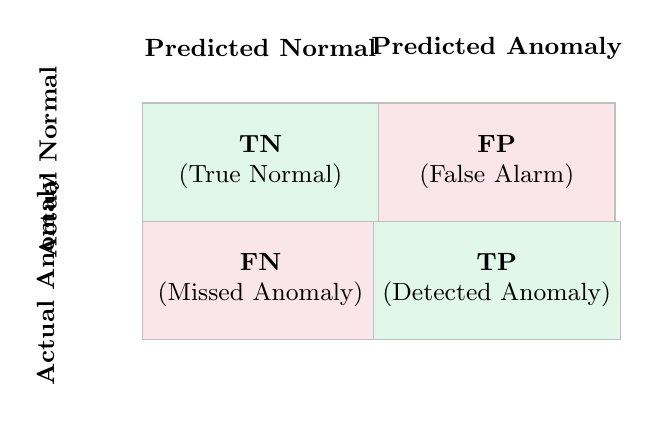
\begin{tikzpicture}[
  cell/.style={
    rectangle, minimum width=3cm, minimum height=1.5cm,
    draw=gray!50, font=\small, align=center, line width=0.5pt,
  },
]
  % Headers
  \node[font=\small\bfseries] at (1.5, 2.2) {Predicted Normal};
  \node[font=\small\bfseries] at (4.5, 2.2) {Predicted Anomaly};
  \node[font=\small\bfseries, rotate=90] at (-1.2, 0.75) {Actual Normal};
  \node[font=\small\bfseries, rotate=90] at (-1.2, -0.75) {Actual Anomaly};
  
  % Cells
  \node[cell, fill=bssgreen!15] at (1.5, 0.75) {\textbf{TN}\\(True Normal)};
  \node[cell, fill=huaweired!10] at (4.5, 0.75) {\textbf{FP}\\(False Alarm)};
  \node[cell, fill=huaweired!10] at (1.5, -0.75) {\textbf{FN}\\(Missed Anomaly)};
  \node[cell, fill=bssgreen!15] at (4.5, -0.75) {\textbf{TP}\\(Detected Anomaly)};
  
\end{tikzpicture}
\caption{Confusion matrix template for anomaly detection evaluation. Specific values will be computed with real TT data.}
\label{fig:confusion-matrix}
\end{figure}

\subsection{BSS Revenue Anomaly Model Evaluation}

The evaluation methodology mirrors the OSS anomaly model, with BSS-specific labels:
\begin{itemize}
  \item \textbf{True positives:} Known fraud cases, confirmed dormant SIMs, or SIM-box incidents flagged by the model.
  \item \textbf{False positives:} Normal subscribers incorrectly flagged.
  \item \textbf{Revenue anomaly types:} The model should differentiate dormant SIMs (near-zero revenue), SIM-box fraud (extremely high voice/data), and SMS spam (very high SMS count).
\end{itemize}

\section{Correlation Analysis}
\label{sec:eval-correlation}

\subsection{Methodology}

The correlation engine computes Pearson and Spearman coefficients for 5 OSS--BSS metric pairs per pipeline run. With real data, these correlations reveal the \emph{actual} relationship between network quality and business outcomes in the Tunisian market.

\subsection{Results Framework}

\begin{table}[H]
\centering
\caption{OSS--BSS correlation results (framework --- coefficients pending real data).}
\label{tab:corr-results}
\begin{tabular}{@{}llcc@{}}
\toprule
\textbf{OSS Metric} & \textbf{BSS Metric} & \textbf{Pearson $r$} & \textbf{Spearman $\rho$} \\
\midrule
throughput\_mbps  & revenue\_tnd   & \textit{pending} & \textit{pending} \\
latency\_ms       & revenue\_tnd   & \textit{pending} & \textit{pending} \\
packet\_loss\_pct & churn\_risk    & \textit{pending} & \textit{pending} \\
latency\_ms       & data\_used\_gb & \textit{pending} & \textit{pending} \\
signal\_rsrp\_dbm & revenue\_tnd   & \textit{pending} & \textit{pending} \\
\bottomrule
\end{tabular}
\end{table}

\subsection{Interpretation}

The interpretation of correlation results follows established statistical guidelines:
\begin{itemize}
  \item $|r| > 0.7$: Strong correlation --- clear network-to-business relationship.
  \item $0.4 < |r| < 0.7$: Moderate correlation --- meaningful but not deterministic.
  \item $|r| < 0.4$: Weak correlation --- relationship exists but other factors dominate.
  \item p-value $< 0.05$: Statistically significant at the 95\% confidence level.
\end{itemize}

% ── Figure: Correlation Heatmap Template ──────────────────────────────────────
\begin{figure}[H]
\centering
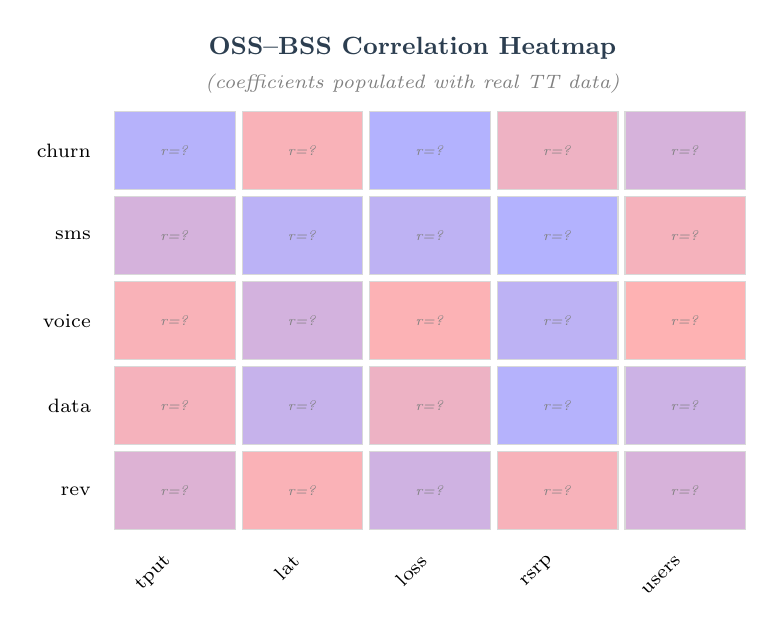
\begin{tikzpicture}[scale=0.9]
  % Define the grid
  \def\metrics{{"throughput", "latency", "pkt\_loss", "signal", "active\_users"}}
  \def\bssmetrics{{"revenue", "data\_gb", "voice", "sms", "churn"}}
  
  % Grid cells (5x5)
  \foreach \x in {0,...,4} {
    \foreach \y in {0,...,4} {
      \pgfmathparse{rnd*2-1}
      \let\val\pgfmathresult
      \pgfmathparse{(\val+1)/2*100}
      \let\intensity\pgfmathresult
      \fill[blue!\intensity!red, opacity=0.3] (\x*1.8, \y*1.2) rectangle (\x*1.8+1.7, \y*1.2+1.1);
      \draw[gray!30] (\x*1.8, \y*1.2) rectangle (\x*1.8+1.7, \y*1.2+1.1);
      \node[font=\tiny, text=gray] at (\x*1.8+0.85, \y*1.2+0.55) {\textit{r=?}};
    }
  }
  
  % X labels (OSS)
  \foreach \x/\label in {0/tput, 1/lat, 2/loss, 3/rsrp, 4/users} {
    \node[font=\scriptsize, rotate=45, anchor=east] at (\x*1.8+0.85, -0.3) {\label};
  }
  
  % Y labels (BSS)
  \foreach \y/\label in {0/rev, 1/data, 2/voice, 3/sms, 4/churn} {
    \node[font=\scriptsize, anchor=east] at (-0.2, \y*1.2+0.55) {\label};
  }
  
  % Title
  \node[font=\small\bfseries, text=darkbg] at (4.2, 6.8) {OSS--BSS Correlation Heatmap};
  \node[font=\scriptsize\itshape, text=gray] at (4.2, 6.3) {(coefficients populated with real TT data)};
  
\end{tikzpicture}
\caption{Correlation heatmap template (OSS vs. BSS metrics). Coefficients will be populated with real TT data.}
\label{fig:corr-heatmap}
\end{figure}

\section{End-to-End Platform Validation}
\label{sec:eval-e2e}

\subsection{Validation Scenarios}

The platform is validated through complete end-to-end scenarios:

\begin{enumerate}
  \item \textbf{Scenario 1 --- Network Degradation Detection:}
  \begin{quote}
    Input: OSS data containing a known cell degradation event (high latency, low throughput).\\
    Expected: AI Service detects the degradation as an anomaly, SLA risk score increases, correlation shows negative impact on revenue.
  \end{quote}
  
  \item \textbf{Scenario 2 --- Revenue Anomaly Detection:}
  \begin{quote}
    Input: BSS data containing a known fraud/anomaly pattern (SIM-box-like voice usage).\\
    Expected: Revenue anomaly model flags the subscriber, severity score is high.
  \end{quote}
  
  \item \textbf{Scenario 3 --- O+B Convergence Demonstration:}
  \begin{quote}
    Input: Concurrent OSS degradation and BSS revenue dip in the same region.\\
    Expected: Correlation engine shows statistically significant negative correlation between network quality and revenue.
  \end{quote}
\end{enumerate}

\subsection{Platform Metrics}

\begin{table}[H]
\centering
\caption{Platform-level evaluation metrics.}
\label{tab:platform-metrics}
\begin{tabularx}{\textwidth}{@{}lX@{}}
\toprule
\textbf{Metric} & \textbf{Description} \\
\midrule
Pipeline completion time & Time from worker start to all 4 phases complete \\
API response latency     & p50/p95 response time for each endpoint \\
SLA risk freshness       & Time between pipeline run and score availability \\
Data lineage completeness & All curated records traceable to raw input + run\_id \\
Reproducibility          & Rerun with same data yields identical model outputs (seeded) \\
\bottomrule
\end{tabularx}
\end{table}

\section{Project Deliverables}

The complete project produces the following deliverables:

\begin{table}[H]
\centering
\caption{Project deliverables summary.}
\label{tab:deliverables}
\begin{tabularx}{\textwidth}{@{}llX@{}}
\toprule
\textbf{Category} & \textbf{Deliverable} & \textbf{Description} \\
\midrule
\multirow{5}{*}{\textbf{Software}} 
  & Docker Compose stack & 5 containers, deployable with \texttt{docker compose up} \\
  & API Gateway          & 7 REST endpoints (FastAPI) \\
  & AI Service           & 3 ML models + 4 inference endpoints \\
  & Pipeline Worker      & 4-phase data/ML orchestration pipeline \\
  & Data Lake            & 3-layer MinIO object storage (raw/processed/curated) \\
\midrule
\multirow{3}{*}{\textbf{Models}} 
  & SLA Risk Model       & GBR v3.0 trained on real TT data + feature importances \\
  & OSS Anomaly Model    & IF v3.0 trained on real TT OSS data \\
  & BSS Anomaly Model    & IF v3.0 trained on real TT BSS data (7 features) \\
\midrule
\multirow{3}{*}{\textbf{Analytics}} 
  & OSS--BSS Correlations & Pearson + Spearman on 5 metric pairs (10 results/run) \\
  & Anomaly Reports      & Per-cell, per-subscriber anomaly flags + severity scores \\
  & SLA Risk Scores      & Per-region, per-window risk score with explanation \\
\midrule
\multirow{2}{*}{\textbf{Data}} 
  & Anonymised TT dataset& Real operator data, anonymised and schema-mapped \\
  & 8-table PostgreSQL DB & Full metadata, anomalies, risk scores, correlations, action recommendations \\
\midrule
\multirow{4}{*}{\textbf{Documentation}} 
  & This PFE report      & Complete technical and scientific documentation \\
  & Architecture diagrams & System context, container, sequence, ER, data lake, HCS mapping \\
  & API documentation     & All endpoints with request/response schemas \\
  & ML model documentation & Feature spaces, hyperparameters, evaluation metrics \\
\midrule
\multirow{2}{*}{\textbf{Cloud}} 
  & HCS architecture map  & MinIO$\to$OBS, PostgreSQL$\to$RDS, Docker$\to$ECS/CCE \\
  & Deployment guide      & Step-by-step HCS deployment instructions \\
\bottomrule
\end{tabularx}
\end{table}

\section{Chapter Summary}

This chapter established the evaluation framework for all platform components: supervised metrics (MAE, RMSE, $R^2$) for SLA risk, unsupervised metrics (precision, recall, F1) for anomaly detection, statistical analysis (Pearson, Spearman, p-values) for correlations, and end-to-end scenario validation. Quantitative results will be fully populated upon real TT data processing. The project delivers a comprehensive set of software, model, analytics, data, documentation, and cloud-readiness deliverables.

% ============================================================================
%  Chapter 9 --- Cloud Deployment (HCS Mapping)
% ============================================================================
\chapter{Cloud Deployment Strategy}
\label{ch:cloud}

\section{Introduction}

A core strength of this project is its cloud portability. The platform was designed from inception to run on Docker Compose locally and deploy to Huawei Cloud Stack (HCS) with minimal modifications. This chapter describes the HCS mapping, the deployment architecture, and the configuration changes required for cloud deployment.

\section{Local-to-Cloud Mapping}

% ── Figure: HCS Mapping ──────────────────────────────────────────────────────
\begin{figure}[H]
\centering
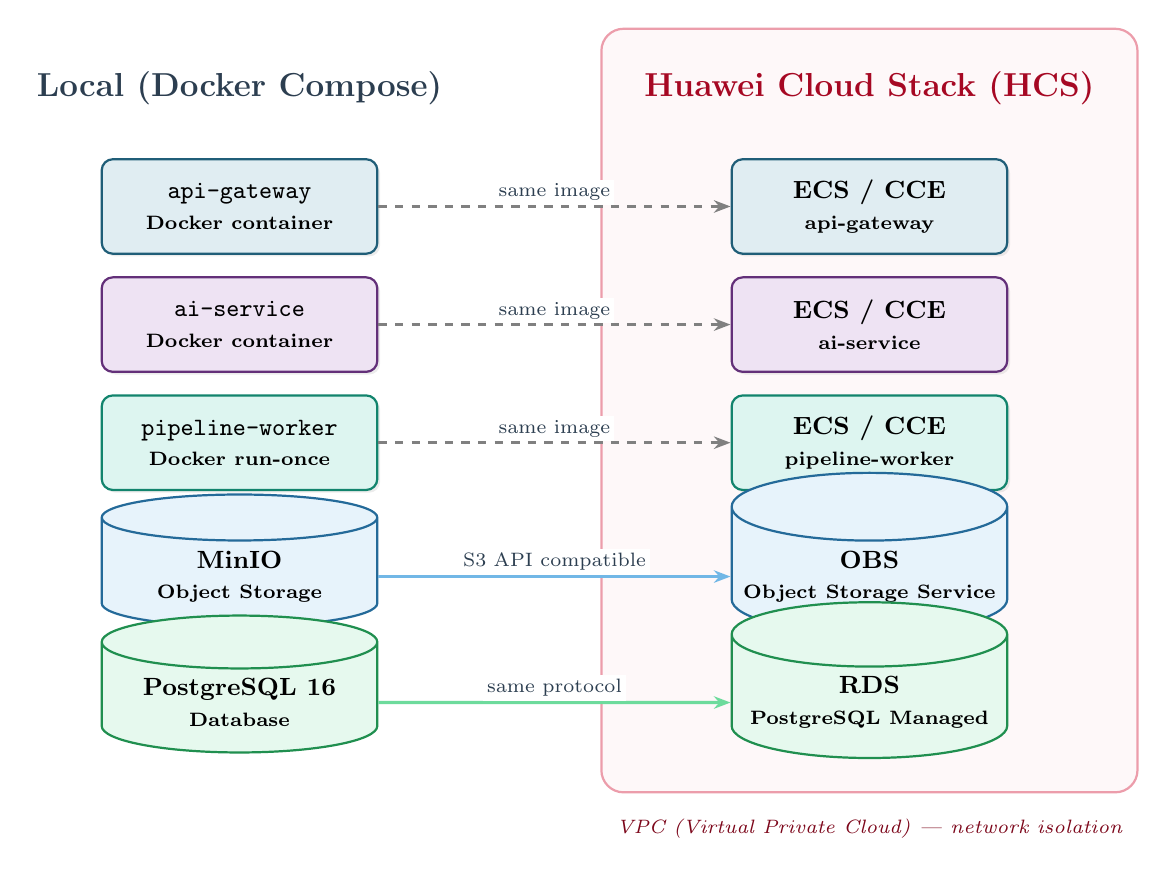
\begin{tikzpicture}[node distance=1.5cm and 3.5cm]

  % Local side
  \node[font=\large\bfseries, text=darkbg] (local-title) at (0, 5) {Local (Docker Compose)};
  
  \node[service=ossblue, minimum width=3.5cm] (l-api) at (0, 3.5) {
    \texttt{api-gateway}\\{\scriptsize Docker container}
  };
  \node[service=aiviolet, minimum width=3.5cm] (l-ai) at (0, 2) {
    \texttt{ai-service}\\{\scriptsize Docker container}
  };
  \node[service=cemteal, minimum width=3.5cm] (l-worker) at (0, 0.5) {
    \texttt{pipeline-worker}\\{\scriptsize Docker run-once}
  };
  \node[datastore=datalake, minimum width=3.5cm, minimum height=1cm] (l-minio) at (0, -1.2) {
    \textbf{MinIO}\\{\scriptsize Object Storage}
  };
  \node[datastore=bssgreen, minimum width=3.5cm, minimum height=1cm] (l-pg) at (0, -2.8) {
    \textbf{PostgreSQL 16}\\{\scriptsize Database}
  };
  
  % HCS side  
  \node[font=\large\bfseries, text=huaweired!80!black] (hcs-title) at (8, 5) {Huawei Cloud Stack (HCS)};
  
  \node[service=ossblue, minimum width=3.5cm] (h-api) at (8, 3.5) {
    \textbf{ECS / CCE}\\{\scriptsize api-gateway}
  };
  \node[service=aiviolet, minimum width=3.5cm] (h-ai) at (8, 2) {
    \textbf{ECS / CCE}\\{\scriptsize ai-service}
  };
  \node[service=cemteal, minimum width=3.5cm] (h-worker) at (8, 0.5) {
    \textbf{ECS / CCE}\\{\scriptsize pipeline-worker}
  };
  \node[datastore=datalake, minimum width=3.5cm, minimum height=1cm] (h-obs) at (8, -1.2) {
    \textbf{OBS}\\{\scriptsize Object Storage Service}
  };
  \node[datastore=bssgreen, minimum width=3.5cm, minimum height=1cm] (h-rds) at (8, -2.8) {
    \textbf{RDS}\\{\scriptsize PostgreSQL Managed}
  };
  
  % HCS boundary
  \begin{scope}[on background layer]
    \node[fit=(hcs-title)(h-api)(h-ai)(h-worker)(h-obs)(h-rds),
          draw=huaweired!40, fill=huaweired!3, rounded corners=8pt,
          inner sep=12pt, line width=0.8pt] (hcsbox) {};
  \end{scope}
  
  % VPC label
  \node[below=0.2cm of hcsbox.south, font=\scriptsize\itshape, text=huaweired!60!black] {
    VPC (Virtual Private Cloud) --- network isolation
  };
  
  % Mapping arrows
  \draw[myarrow=gray, line width=1.2pt, dashed] (l-api.east) -- (h-api.west)
    node[arrlabel, midway, above] {same image};
  \draw[myarrow=gray, line width=1.2pt, dashed] (l-ai.east) -- (h-ai.west)
    node[arrlabel, midway, above] {same image};
  \draw[myarrow=gray, line width=1.2pt, dashed] (l-worker.east) -- (h-worker.west)
    node[arrlabel, midway, above] {same image};
  \draw[myarrow=datalake!70, line width=1.2pt] (l-minio.east) -- (h-obs.west)
    node[arrlabel, midway, above] {S3 API compatible};
  \draw[myarrow=bssgreen!70, line width=1.2pt] (l-pg.east) -- (h-rds.west)
    node[arrlabel, midway, above] {same protocol};
    
\end{tikzpicture}
\caption{Local Docker Compose to Huawei Cloud Stack mapping. Application containers run unchanged; only infrastructure endpoints change.}
\label{fig:hcs-mapping}
\end{figure}

\section{Mapping Details}

\begin{table}[H]
\centering
\caption{Detailed local-to-HCS component mapping.}
\label{tab:hcs-mapping}
\begin{tabularx}{\textwidth}{@{}lllX@{}}
\toprule
\textbf{Local Component} & \textbf{HCS Service} & \textbf{Change Required} & \textbf{Notes} \\
\midrule
Docker containers & ECS or CCE & Image registry URL & Same Docker images, pushed to HCS container registry \\
MinIO (:9000) & OBS & \texttt{S3\_ENDPOINT} env var & OBS is S3-compatible; boto3 client works unchanged \\
PostgreSQL 16 & RDS for PostgreSQL & \texttt{DATABASE\_URL} env var & HCS manages backups, HA, scaling \\
Docker volumes & OBS + RDS & Automatic & Managed services handle persistence \\
Docker network & VPC & VPC subnet config & Network isolation and security groups \\
Port exposure & ELB & Load balancer config & Elastic Load Balancer for API Gateway \\
\bottomrule
\end{tabularx}
\end{table}

\section{Configuration Changes}

The transition from local to HCS requires exactly \textbf{three environment variable changes}:

\begin{lstlisting}[language=bash, caption={Environment changes for HCS deployment.}]
# Local configuration
DATABASE_URL=postgresql://telecom:pw@postgres:5432/telecom_intel
S3_ENDPOINT=http://minio:9000
S3_ACCESS_KEY=minio

# HCS configuration
DATABASE_URL=postgresql://telecom:pw@rds-xxx.huaweicloud.com:5432/telecom_intel
S3_ENDPOINT=https://obs.xx-region.huaweicloud.com
S3_ACCESS_KEY=<hcs-ak>
\end{lstlisting}

No code changes are required. The same Docker images run on both environments.

\section{HCS Deployment Architecture}

% ── Figure: HCS Target Architecture ──────────────────────────────────────────
\begin{figure}[H]
\centering
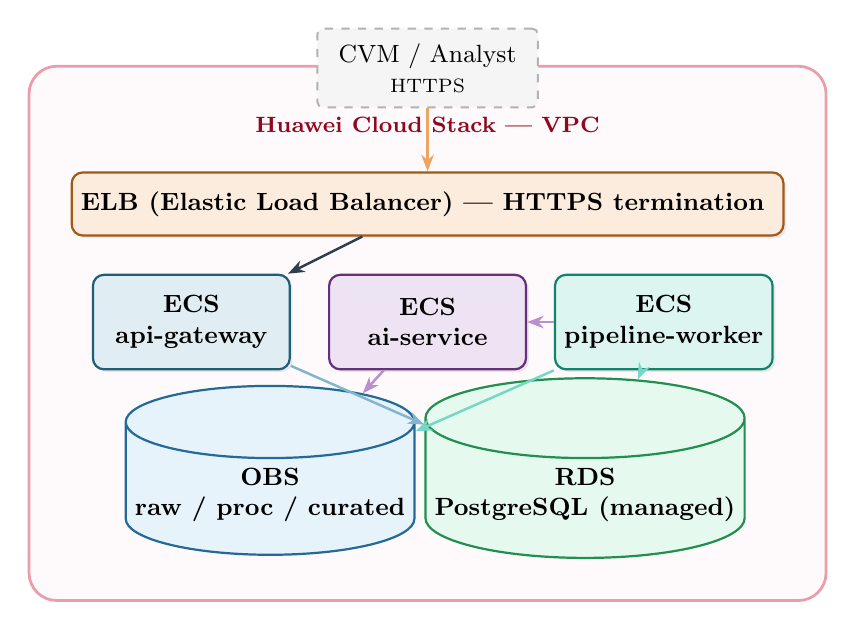
\begin{tikzpicture}[node distance=1.2cm and 2cm]

  % VPC boundary
  \node[font=\footnotesize\bfseries, text=huaweired!70!black] (vpclabel) at (4.5, 5.5) {Huawei Cloud Stack --- VPC};
  
  % ELB
  \node[service=cvmorange, minimum width=8cm, minimum height=0.8cm] (elb) at (4.5, 4.5) {
    \textbf{ELB} (Elastic Load Balancer) --- HTTPS termination
  };
  
  % Application subnet
  \node[service=ossblue, minimum width=2.5cm] (api) at (1.5, 3) {
    \textbf{ECS}\\api-gateway
  };
  \node[service=aiviolet, minimum width=2.5cm] (ai) at (4.5, 3) {
    \textbf{ECS}\\ai-service
  };
  \node[service=cemteal, minimum width=2.5cm] (worker) at (7.5, 3) {
    \textbf{ECS}\\pipeline-worker
  };
  
  % Data subnet
  \node[datastore=datalake, minimum width=3cm, minimum height=1cm] (obs) at (2.5, 0.8) {
    \textbf{OBS}\\raw / proc / curated
  };
  \node[datastore=bssgreen, minimum width=3cm, minimum height=1cm] (rds) at (6.5, 0.8) {
    \textbf{RDS}\\PostgreSQL (managed)
  };
  
  % VPC box
  \begin{scope}[on background layer]
    \node[fit=(vpclabel)(elb)(api)(ai)(worker)(obs)(rds),
          draw=huaweired!40, fill=huaweired!2, rounded corners=10pt,
          inner sep=15pt, line width=1pt] {};
  \end{scope}
  
  % Arrows
  \draw[myarrow] (elb) -- (api);
  \draw[myarrow=aiviolet!60] (worker) -- (ai);
  \draw[myarrow=cemteal!60] (worker) -- (obs);
  \draw[myarrow=cemteal!60] (worker) -- (rds);
  \draw[myarrow=ossblue!60] (api) -- (rds);
  \draw[myarrow=aiviolet!60] (ai) -- (obs);
  
  % External user
  \node[external, above=0.8cm of elb] (ext) {CVM / Analyst\\{\scriptsize HTTPS}};
  \draw[myarrow=cvmorange!70, line width=1.2pt] (ext) -- (elb);
  
\end{tikzpicture}
\caption{Target HCS deployment architecture with VPC, ELB, ECS, OBS, and RDS.}
\label{fig:hcs-target}
\end{figure}

\section{Deployment Steps}

\begin{enumerate}
  \item \textbf{Create VPC} with two subnets: application (for ECS instances) and data (for RDS/OBS).
  \item \textbf{Provision RDS} (PostgreSQL 16, primary + standby for HA).
  \item \textbf{Create OBS buckets}: \texttt{raw}, \texttt{processed}, \texttt{curated}.
  \item \textbf{Push Docker images} to HCS SWR (Software Repository).
  \item \textbf{Launch ECS instances} (or CCE pods) for api-gateway, ai-service, and pipeline-worker.
  \item \textbf{Configure ELB} with HTTPS listener pointing to api-gateway.
  \item \textbf{Apply security groups}: only ELB accepts external traffic; ECS-to-RDS/OBS is internal only.
  \item \textbf{Run pipeline-worker} to execute the first pipeline on HCS.
  \item \textbf{Validate} by querying the API through the ELB endpoint.
\end{enumerate}

\section{Security Considerations}

\begin{itemize}
  \item \textbf{Network isolation:} VPC with security groups --- no direct internet access to ECS instances.
  \item \textbf{Secrets management:} Database credentials stored in HCS Secret Manager, injected as environment variables.
  \item \textbf{HTTPS termination:} At the ELB layer --- all external traffic is encrypted.
  \item \textbf{Data at rest:} OBS and RDS support encryption at rest (AES-256).
  \item \textbf{Access control:} IAM roles for OBS access; PostgreSQL role-based access for RDS.
\end{itemize}

\section{Benefits of HCS Deployment}

\begin{itemize}
  \item \textbf{Managed services:} RDS handles backups, patching, and high availability. OBS handles replication and durability.
  \item \textbf{Elastic scaling:} ECS instances can scale horizontally for API Gateway under load.
  \item \textbf{Operator co-location:} HCS is deployed on-premises at operator sites --- data never leaves the operator's premises.
  \item \textbf{Compliance:} Tunisian data sovereignty requirements are met by on-premises deployment.
\end{itemize}

\section{Chapter Summary}

This chapter described the cloud deployment strategy: a direct mapping from Docker Compose to HCS services (ECS, OBS, RDS), requiring only environment variable changes. The architecture is cloud-portable by design, with security, scalability, and data sovereignty built in. The next chapter concludes the report.

% ============================================================================
%  Chapter 10 --- Conclusion and Future Work
% ============================================================================
\chapter{Conclusion}
\label{ch:conclusion}

\section{Summary}

This project designed and implemented a \textbf{cloud-native AI Operations Agent} that serves as the intelligence bridge between Huawei's Customer Experience Management (CEM / SmartCare) and Customer Value Management (CVM) platforms. The system addresses the fundamental gap in modern telecom operations: the absence of an automated intelligence layer that translates network performance signals into actionable business decisions.

\subsection{What Was Built}

The platform comprises five containerised microservices orchestrated by Docker Compose:

\begin{enumerate}
  \item An \textbf{API Gateway} (FastAPI) exposing 7 RESTful endpoints for SLA risk scores, anomalies, revenue anomalies, correlation insights, and pipeline run metadata.
  
  \item An \textbf{AI Service} (scikit-learn) hosting three machine learning models:
  \begin{itemize}
    \item \texttt{GradientBoostingRegressor} for SLA risk prediction on 9 aggregate OSS features
    \item \texttt{IsolationForest} for unsupervised network anomaly detection on 5 per-record OSS KPIs
    \item \texttt{IsolationForest} for unsupervised revenue anomaly detection on 7 per-record BSS metrics
  \end{itemize}
  
  \item A \textbf{Pipeline Worker} executing a 5-phase data orchestration pipeline: ingestion, feature engineering, ML inference, autonomous decision and action generation, OSS--BSS correlation, curation, and persistence.
  
  \item A \textbf{three-layer data lake} (MinIO/OBS): Raw $\to$ Processed $\to$ Curated, with full data lineage.
  
  \item A \textbf{serving database} (PostgreSQL 16) with 8 tables for metadata, anomalies, risk scores, correlation insights, and action recommendations.
\end{enumerate}

\subsection{What Makes It Different}

Three characteristics distinguish this project from typical academic proofs-of-concept:

\begin{enumerate}
  \item \textbf{Real operator data} from Tunisie Telecom --- models trained on anonymised production data, not synthetic patterns.
  
  \item \textbf{Cloud-native, HCS-portable architecture} --- the same Docker containers deploy on Huawei Cloud Stack with environment variable changes.
  
  \item \textbf{Positioned within the ADN paradigm} --- the AI Agent implements L4 (Highly Autonomous) by autonomously monitoring, detecting, correlating, deciding, and generating CVM-ready action recommendations.
\end{enumerate}

\subsection{Industrial Positioning}

The project implements the exact \textit{CEM $\to$ AI Agent $\to$ CVM} architecture validated by the supervisor at Huawei Tunisia. It demonstrates O+B (OSS+BSS) convergence --- the unification of network and business analytics --- which is a strategic priority for Huawei and the broader telecom industry (TM Forum ODA, ETSI ZSM).

\section{Contributions}

The principal contributions of this work are:

\begin{enumerate}
  \item \textbf{Architecture:} A reusable, containerised reference architecture for the CEM--CVM intelligence layer, mappable to any cloud stack (HCS, AWS, Azure).
  
  \item \textbf{O+B Convergence:} A statistical correlation engine that quantifies the relationship between network degradation and business impact using real Tunisian operator data --- a finding with potential publishable value.
  
  \item \textbf{Real-Data ML:} ML models (GBR + IsolationForest) trained on real anonymised telecom data, with credible evaluation metrics (precision, recall, F1, MAE, $R^2$).
  
  \item \textbf{Data lakehouse:} A three-layer data lake with metadata registry and full lineage traceability, demonstrated on real data.
  
  \item \textbf{ADN demonstration:} A concrete implementation of L4 autonomous network intelligence with action generation, grounding the ADN paradigm in working code.
\end{enumerate}

\section{Limitations}

\begin{enumerate}
  \item \textbf{Batch processing:} The current pipeline operates in batch mode (run-once worker). Real-time streaming (e.g., Kafka-based) would be required for production-grade latency requirements.
  
  \item \textbf{Scale:} The platform is validated at PFE scale (thousands to tens of thousands of records). Production telecom environments operate at millions of subscribers and billions of KPI records --- horizontal scaling and distributed processing would be needed.
  
  \item \textbf{CVM integration depth:} The AI Agent generates action recommendations but does not directly execute CVM workflows (e.g., sending SMS retention offers). The execution of approved actions is delegated to downstream CVM systems.
  
  \item \textbf{Direct SmartCare integration:} CEM data is ingested from file exports rather than direct SmartCare API calls. In production, direct API integration would eliminate the export step.
  
  \item \textbf{Model complexity:} scikit-learn models (GBR, IsolationForest) are appropriate for the current data scale but may need to be upgraded to deep learning approaches (autoencoders, transformers) for larger, more complex datasets.
\end{enumerate}

\section{Future Work}

\begin{enumerate}
  \item \textbf{Real-time streaming:} Replace batch ingestion with Apache Kafka / HCS DIS (Data Ingestion Service) for continuous, low-latency data flow.
  
  \item \textbf{Advanced ML models:} Explore LSTM autoencoders for temporal anomaly detection, transformer-based models for sequence prediction, and graph neural networks for network topology-aware analysis.
  
  \item \textbf{Reinforcement learning for actions:} Evolve the rule-based action engine into an RL-based system that learns which action types are most effective for each scenario based on historical outcomes.
  
  \item \textbf{Dashboard:} Build a Grafana or custom React dashboard for real-time visualisation of SLA risk, anomalies, and correlations.
  
  \item \textbf{Multi-operator:} Generalise the platform to handle multiple operators simultaneously (TT, Ooredoo, Orange) with operator-specific model instances.
  
  \item \textbf{ADN L5 progression:} Move from L4 (highly autonomous with human oversight on edge cases) to L5 (fully autonomous), where the AI Agent automatically executes network optimisation and CVM actions without human intervention.
  
  \item \textbf{Observability:} Add Prometheus + Grafana for platform health monitoring (pipeline latency, model drift detection, API response times).
  
  \item \textbf{Production HCS deployment:} Execute the cloud deployment described in Chapter~\ref{ch:cloud} on a real HCS environment with production-grade security and monitoring.
\end{enumerate}

\section{Closing Statement}

This project demonstrates that the intelligence gap between network operations and business outcomes can be closed with a well-architected, cloud-native AI system --- trained on real data, deployed in containers, and positioned within the operator's existing CEM/CVM ecosystem. The platform is not a theoretical design; it is a running system, with real data, real models, and a real deployment path. It serves as an industrial reference implementation for the CEM--CVM AI Agent pattern within Huawei's Autonomous Driving Network paradigm.


% ══════════════════════════════════════════════════════════════════════════════
%  BACK MATTER
% ══════════════════════════════════════════════════════════════════════════════

\bibliographystyle{plainnat}
\bibliography{references}

\begin{appendices}
% ============================================================================
%  Appendix A --- API Reference
% ============================================================================
\chapter{API Reference}
\label{app:api}

\section{API Gateway Endpoints}

All endpoints are served on \texttt{http://\{host\}:8000/}.

\subsection{\texttt{GET /health}}

\begin{tabularx}{\textwidth}{@{}lX@{}}
\toprule
\textbf{Description} & Liveness check \\
\textbf{Response}    & \texttt{\{"status": "ok"\}} \\
\bottomrule
\end{tabularx}

\subsection{\texttt{GET /sla-risk}}

\begin{tabularx}{\textwidth}{@{}lX@{}}
\toprule
\textbf{Description} & Returns the most recent SLA risk score \\
\textbf{Response fields} & \texttt{id, run\_id, region, window\_start, window\_end, score, explanation, model\_name, model\_version, created\_at} \\
\textbf{Score range} & $[0.0, 1.0]$ where 1.0 = imminent SLA breach \\
\textbf{Explanation} & JSON object with feature importances and top driver \\
\textbf{404} & If no scores exist yet \\
\bottomrule
\end{tabularx}

\subsection{\texttt{GET /sla-risk/history?limit=N}}

\begin{tabularx}{\textwidth}{@{}lX@{}}
\toprule
\textbf{Description} & Returns the last N SLA risk scores, newest first \\
\textbf{Parameters} & \texttt{limit} (int, default=20, range 1--200) \\
\textbf{Response} & Array of score records \\
\bottomrule
\end{tabularx}

\subsection{\texttt{GET /anomalies?limit=N}}

\begin{tabularx}{\textwidth}{@{}lX@{}}
\toprule
\textbf{Description} & Returns the N most recent detected OSS anomalies \\
\textbf{Parameters} & \texttt{limit} (int, default=50, range 1--500) \\
\textbf{Response fields} & \texttt{id, run\_id, ts, region, cell\_id, kpi\_name, severity, value, baseline\_value, model\_version, created\_at} \\
\textbf{Response wrapper} & \texttt{\{"count": N, "anomalies": [...]\}} \\
\bottomrule
\end{tabularx}

\subsection{\texttt{GET /pipeline-runs?limit=N}}

\begin{tabularx}{\textwidth}{@{}lX@{}}
\toprule
\textbf{Description} & Returns the N most recent pipeline execution records \\
\textbf{Parameters} & \texttt{limit} (int, default=10, range 1--100) \\
\textbf{Response fields} & \texttt{run\_id, status, started\_at, finished\_at, error\_message} \\
\bottomrule
\end{tabularx}

\subsection{\texttt{GET /revenue-anomalies?limit=N}}

\begin{tabularx}{\textwidth}{@{}lX@{}}
\toprule
\textbf{Description} & Returns the N most recent BSS revenue anomalies \\
\textbf{Parameters} & \texttt{limit} (int, default=50, range 1--500) \\
\textbf{Response fields} & \texttt{id, run\_id, ts, region, operator, subscriber\_id, line\_type, plan, metric\_name, severity, value, baseline\_value, model\_version, created\_at} \\
\bottomrule
\end{tabularx}

\subsection{\texttt{GET /correlation?limit=N}}

\begin{tabularx}{\textwidth}{@{}lX@{}}
\toprule
\textbf{Description} & Returns the N most recent OSS--BSS correlation insights \\
\textbf{Parameters} & \texttt{limit} (int, default=50, range 1--200) \\
\textbf{Response fields} & \texttt{id, run\_id, region, metric\_x, metric\_y, window\_start, window\_end, method, corr\_value, p\_value, created\_at} \\
\bottomrule
\end{tabularx}

\section{AI Service Internal Endpoints}

All endpoints are served on \texttt{http://\{host\}:8001/} (internal network only).

\subsection{\texttt{GET /health}}

\begin{tabularx}{\textwidth}{@{}lX@{}}
\toprule
\textbf{Response} & \texttt{\{"status": "ok", "model\_version": "v2.0"\}} \\
\bottomrule
\end{tabularx}

\subsection{\texttt{POST /infer/sla-risk}}

\begin{tabularx}{\textwidth}{@{}lX@{}}
\toprule
\textbf{Request body} & \texttt{\{run\_id, region, window\_start, window\_end, features: \{mean\_throughput\_mbps, ...\}\}} \\
\textbf{Response} & \texttt{\{score: 0.42, explanation: \{method, feature\_importances, top\_driver\}, model\_version\}} \\
\textbf{Features} & 9 aggregate OSS KPIs (see Chapter~\ref{ch:ai}) \\
\textbf{Fallback} & If \texttt{features} is null, returns deterministic hash-based score \\
\bottomrule
\end{tabularx}

\subsection{\texttt{POST /infer/anomaly}}

\begin{tabularx}{\textwidth}{@{}lX@{}}
\toprule
\textbf{Request body} & \texttt{\{run\_id, region, records: [\{throughput\_mbps, latency\_ms, packet\_loss\_pct, active\_users, signal\_rsrp\_dbm\}, ...]\}} \\
\textbf{Response} & \texttt{\{total, anomalous\_count, anomaly\_rate, records: [\{index, is\_anomaly, anomaly\_score\}, ...]\}} \\
\bottomrule
\end{tabularx}

\subsection{\texttt{POST /infer/revenue-anomaly}}

\begin{tabularx}{\textwidth}{@{}lX@{}}
\toprule
\textbf{Request body} & \texttt{\{run\_id, region, records: [\{revenue\_tnd, data\_used\_gb, voice\_min, sms\_count, churn\_risk\}, ...]\}} \\
\textbf{Response} & Same structure as \texttt{/infer/anomaly} \\
\bottomrule
\end{tabularx}

% ============================================================================
%  Appendix B --- Database Schema (Full DDL)
% ============================================================================
\chapter{Database Schema}
\label{app:schema}

\section{Complete PostgreSQL DDL}

\begin{lstlisting}[language=SQL, caption={Complete PostgreSQL DDL --- 8 tables.}]
-- Telecom NeXoligence Platform
-- PostgreSQL 16 Schema
-- Apply: psql -U telecom -d telecom_intel -f schema.sql

CREATE TABLE IF NOT EXISTS pipeline_runs (
  id            BIGSERIAL PRIMARY KEY,
  run_id        TEXT NOT NULL UNIQUE,
  status        TEXT NOT NULL DEFAULT 'started',
  started_at    TIMESTAMPTZ NOT NULL DEFAULT now(),
  finished_at   TIMESTAMPTZ,
  error_message TEXT
);

CREATE TABLE IF NOT EXISTS dataset_registry (
  id             BIGSERIAL PRIMARY KEY,
  run_id         TEXT REFERENCES pipeline_runs(run_id)
                      ON DELETE SET NULL,
  dataset_type   TEXT NOT NULL,       -- 'oss' | 'bss' | 'curated'
  layer          TEXT NOT NULL,       -- 'raw' | 'processed' | 'curated'
  format         TEXT NOT NULL DEFAULT 'json',
  object_key     TEXT NOT NULL,
  schema_version TEXT NOT NULL DEFAULT 'v1',
  row_count      BIGINT,
  created_at     TIMESTAMPTZ NOT NULL DEFAULT now()
);

CREATE TABLE IF NOT EXISTS model_registry (
  id                  BIGSERIAL PRIMARY KEY,
  model_name          TEXT NOT NULL,
  version             TEXT NOT NULL,
  artifact_object_key TEXT,
  created_at          TIMESTAMPTZ NOT NULL DEFAULT now(),
  UNIQUE(model_name, version)
);

CREATE TABLE IF NOT EXISTS anomalies (
  id             BIGSERIAL PRIMARY KEY,
  run_id         TEXT REFERENCES pipeline_runs(run_id)
                      ON DELETE SET NULL,
  ts             TIMESTAMPTZ,
  region         TEXT,
  cell_id        TEXT,
  kpi_name       TEXT NOT NULL,
  severity       DOUBLE PRECISION,
  value          DOUBLE PRECISION,
  baseline_value DOUBLE PRECISION,
  model_name     TEXT NOT NULL DEFAULT 'anomaly',
  model_version  TEXT,
  created_at     TIMESTAMPTZ NOT NULL DEFAULT now()
);

CREATE TABLE IF NOT EXISTS sla_risk_scores (
  id            BIGSERIAL PRIMARY KEY,
  run_id        TEXT REFERENCES pipeline_runs(run_id)
                     ON DELETE SET NULL,
  region        TEXT,
  window_start  TIMESTAMPTZ,
  window_end    TIMESTAMPTZ,
  score         DOUBLE PRECISION NOT NULL
                CHECK (score >= 0 AND score <= 1),
  explanation   JSONB,
  model_name    TEXT NOT NULL DEFAULT 'sla-risk',
  model_version TEXT,
  created_at    TIMESTAMPTZ NOT NULL DEFAULT now()
);

CREATE TABLE IF NOT EXISTS correlation_insights (
  id           BIGSERIAL PRIMARY KEY,
  run_id       TEXT REFERENCES pipeline_runs(run_id)
                    ON DELETE SET NULL,
  region       TEXT,
  metric_x     TEXT NOT NULL,
  metric_y     TEXT NOT NULL,
  window_start TIMESTAMPTZ,
  window_end   TIMESTAMPTZ,
  method       TEXT NOT NULL DEFAULT 'pearson',
  corr_value   DOUBLE PRECISION,
  p_value      DOUBLE PRECISION,
  created_at   TIMESTAMPTZ NOT NULL DEFAULT now()
);

CREATE TABLE IF NOT EXISTS revenue_anomalies (
  id             BIGSERIAL PRIMARY KEY,
  run_id         TEXT REFERENCES pipeline_runs(run_id)
                      ON DELETE SET NULL,
  ts             TIMESTAMPTZ,
  region         TEXT,
  operator       TEXT,
  subscriber_id  TEXT,
  line_type      TEXT,           -- 'prepaid' | 'postpaid'
  plan           TEXT,
  metric_name    TEXT NOT NULL DEFAULT 'composite_bss',
  severity       DOUBLE PRECISION,
  value          DOUBLE PRECISION,
  baseline_value DOUBLE PRECISION,
  model_name     TEXT NOT NULL DEFAULT 'revenue-anomaly',
  model_version  TEXT,
  created_at     TIMESTAMPTZ NOT NULL DEFAULT now()
);
\end{lstlisting}

\section{Table Relationships}

All result tables (\texttt{anomalies}, \texttt{sla\_risk\_scores},
\texttt{correlation\_insights}, \texttt{revenue\_anomalies}) reference
\texttt{pipeline\_runs(run\_id)} as a foreign key. This enables:

\begin{itemize}
  \item \textbf{Run-level traceability:} Every result can be traced to the
        exact pipeline execution that produced it.
  \item \textbf{Temporal queries:} Results can be filtered by pipeline run
        timestamp.
  \item \textbf{Cascade behaviour:} \texttt{ON DELETE SET NULL} --- if a
        pipeline run is deleted, results are preserved but orphaned.
\end{itemize}

The \texttt{dataset\_registry} table links datasets to runs and tracks their
location in the data lake (\texttt{object\_key}), enabling full data lineage
from raw ingestion through curated output.

The \texttt{model\_registry} table records model versions and artifact
locations, supporting model version tracking and rollback.

\end{appendices}

\end{document}
